\documentclass[conference]{IEEEtran}
\IEEEoverridecommandlockouts

\usepackage{cite}
\usepackage{amsmath,amssymb,amsfonts}
\usepackage{graphicx}
\usepackage{textcomp}
\usepackage{xcolor}
\usepackage{booktabs}
\usepackage{multirow}
\usepackage{tabularx}
\usepackage{url}
\usepackage[utf8]{inputenc}
\usepackage[T1]{fontenc}
\usepackage{balance}
\usepackage{microtype}
\usepackage{placeins}
\usepackage{flafter}

% Parámetros de posicionamiento de flotantes IEEE
\renewcommand{\topfraction}{0.95}
\renewcommand{\bottomfraction}{0.95}
\renewcommand{\textfraction}{0.05}
\renewcommand{\floatpagefraction}{0.70}
\renewcommand{\dbltopfraction}{0.95}
\renewcommand{\dblfloatpagefraction}{0.70}
\setcounter{topnumber}{4}
\setcounter{bottomnumber}{4}
\setcounter{totalnumber}{8}
\setcounter{dbltopnumber}{4}

\def\BibTeX{{\rm B\kern-.05em{\sc i\kern-.025em b}\kern-.08em
    T\kern-.1667em\lower.7ex\hbox{E}\kern-.125emX}}

\begin{document}

\title{Auditor\'ia de Calidad ISO/IEC 25010 y Modernizaci\'on\\
Ergon\'omica ISO~9241 de un Sistema Legado de Vigilancia\\
Epidemiol\'ogica para Infecciones Respiratorias Agudas}

\author{
  \begin{tabular}{c@{\hspace{1.5em}}c@{\hspace{1.5em}}c}
    \begin{tabular}{@{}c@{}}
      \textbf{Leonardo Ruben Arce Mayhua}\\[0.2ex]
      \small\textit{Universidad Nacional de San Agust\'in}\\
      \small Arequipa, Per\'u\\
      \small\texttt{larcem@unsa.edu.pe}
    \end{tabular} &
    \begin{tabular}{@{}c@{}}
      \textbf{Joel Isaias Condori Leon}\\[0.2ex]
      \small\textit{Universidad Nacional de San Agust\'in}\\
      \small Arequipa, Per\'u\\
      \small\texttt{jcondorile@unsa.edu.pe}
    \end{tabular} &
    \begin{tabular}{@{}c@{}}
      \textbf{Marco Antonio Marquez Herrera}\\[0.2ex]
      \small\textit{Universidad Nacional de San Agust\'in}\\
      \small Arequipa, Per\'u\\
      \small\texttt{mmarquezhe@unsa.edu.pe}
    \end{tabular}
  \end{tabular}\\[1.2em]
  \begin{tabular}{c@{\hspace{3.5em}}c}
    \begin{tabular}{@{}c@{}}
      \textbf{Rafael Diego Nina Calizaya}\\[0.2ex]
      \small\textit{Universidad Nacional de San Agust\'in}\\
      \small Arequipa, Per\'u\\
      \small\texttt{rninacal@unsa.edu.pe}
    \end{tabular} &
    \begin{tabular}{@{}c@{}}
      \textbf{Jeremy Joshua Perez Huamani}\\[0.2ex]
      \small\textit{Universidad Nacional de San Agust\'in}\\
      \small Arequipa, Per\'u\\
      \small\texttt{jperezhua@unsa.edu.pe}
    \end{tabular}
  \end{tabular}
}

\maketitle

\begin{abstract}
Este art\'iculo aplica ingenier\'ia inversa est\'atica y auditor\'ia de calidad de software a \textit{ISPySA-Pneumonia}, un flujo anal\'itico de c\'odigo abierto de 6\,839 l\'ineas en Python para la vigilancia epidemiol\'ogica de Infecciones Respiratorias Agudas (IRA) y neumon\'ia en el Per\'u (2000--2023). Nuestra investigaci\'on aborda tres objetivos fundamentales: (i)~recuperar la topolog\'ia arquitect\'onica por capas y los contratos de datos a partir \'unicamente de los artefactos del c\'odigo fuente; (ii)~identificar, clasificar bajo el est\'andar ISO/IEC~25010 y subsanar los defectos estructurales con los que la publicaci\'on original fue liberada; y (iii)~dise\~nar, implementar y verificar una plataforma interactiva de monitoreo cl\'inico cuya ergonom\'ia visual y arquitectura de interacci\'on se adhieren estrictamente a las normas ISO~9241-11, ISO~9241-210, ISO~9241-110 e ISO~9241-12. La auditor\'ia de ingenier\'ia inversa revel\'o tres defectos cr\'iticos en los contratos de datos: dos rutas de archivos truncadas que causaban el consumo silencioso de datos poblacionales desactualizados, y una incompatibilidad de empaquetado de entorno que inhabilita los modelos LSTM legados. Tras la remediaci\'on, el flujo de preparaci\'on de datos fue reejecutado sobre 2\,143\,985 registros distritales semanales, replicando fielmente las din\'amicas epidemiol\'ogicas publicadas. Para desacoplar la capa de presentaci\'on de la estructura de archivos legada, se dise\~n\'o una capa de servicios anticorrupci\'on (\texttt{EpidemiologyDataService} y \texttt{EpidemiologyModelService}). La plataforma resultante, desarrollada en Streamlit y estilizada mediante Tokens de Dise\~no normalizados y primitivas de UI accesibles, expone cinco m\'odulos de vigilancia cl\'inica con cero emojis informales y codificaci\'on visual redundante conforme a WCAG~AAA. La integridad operacional se verific\'o mediante una suite de pruebas automatizadas que eval\'ua aserciones unitarias, de integraci\'on y de invariantes epidemiol\'ogicas de dominio, alcanzando una tasa de aprobaci\'on del 100\% en 0.053\,s.
\end{abstract}

\begin{IEEEkeywords}
ingenier\'ia inversa, vigilancia epidemiol\'ogica, ISO~9241, ISO/IEC~25010, Streamlit, calidad de software, capa anticorrupci\'on, Python, IRA, neumon\'ia, Per\'u
\end{IEEEkeywords}

\section{Introducci\'on}
\label{sec:intro}

Los sistemas de informaci\'on en salud p\'ublica enfrentan una persistente brecha estructural entre el rigor anal\'itico computacional y los requisitos operacionales de los tomadores de decisiones cl\'inicas. Los flujos anal\'iticos basados en \textit{scripts} aislados---secuencias de archivos procedimentales donde cada rutina ingiere datos tabulares, ejecuta transformaciones y emite archivos planos o gr\'aficos est\'aticos intermedios---est\'an ampliamente extendidos en grupos de investigaci\'on acad\'emica y direcciones regionales de salud con recursos de ingenier\'ia de software limitados~\cite{Feathers2004}. Aunque reproducibles a nivel computacional, estos flujos procedimentales exhiben severas deficiencias de mantenibilidad y usabilidad: las conclusiones anal\'iticas quedan confinadas dentro de \'arboles de directorios inconexos repletos de figuras PNG y tablas CSV que el epidemi\'ologo debe localizar, correlacionar e interpretar manualmente, sin capacidades de consulta din\'amica.

En el Per\'u, las Infecciones Respiratorias Agudas (IRA) y la neumon\'ia constituyen la principal causa de morbimortalidad evitable en cohortes demogr\'aficas vulnerables: ni\~nos menores de cinco a\~nos ($<$5) y adultos mayores de sesenta a\~nos a m\'as (60+)~\cite{PAHO2011}. Los incrementos estacionales est\'an fuertemente condicionados por factores bioclim\'aticos, manifestando profundas disparidades territoriales entre las zonas altoandinas sujetas a intensas heladas y los departamentos amaz\'onicos caracterizados por humedad persistente y aislamiento geogr\'afico. La detecci\'on oportuna de brotes epidemiol\'ogicos an\'omalos es indispensable para la asignaci\'on racional de camas hospitalarias, ox\'igeno medicinal y personal m\'edico entre las Direcciones Regionales de Salud (DIRESA). Cuando las herramientas anal\'iticas no logran exponer paneles interactivos y accesibles, las autoridades sanitarias se ven forzadas a depender de boletines trimestrales extempor\'aneos o del procesamiento manual en hojas de c\'alculo.

El repositorio de c\'odigo abierto \textit{ISPySA-Pneumonia}~\cite{Danala2024} constituye un caso representativo de esta situaci\'on. Dicho sistema provee un an\'alisis hist\'orico exhaustivo sobre incidencia, estacionalidad, jerarquizaci\'on territorial y modelamiento predictivo de las IRA en el Per\'u durante una ventana de 24 a\~nos (2000--2023). No obstante, su utilidad operativa resulta comprometida por una salida dispersa en decenas de gr\'aficos est\'aticos. M\'as cr\'itico a\'un, nuestra auditor\'ia de ingenier\'ia inversa est\'atica descubri\'o que la ausencia de contratos de datos expl\'icitos entre rutinas gener\'o defectos de rutas de archivos que la publicaci\'on original distribuy\'o sin detectar, provocando que los \textit{scripts} subsiguientes consumieran datos desactualizados en silencio.

Para superar estas limitaciones, este art\'iculo documenta un proceso riguroso de ingenier\'ia de calidad de software:
\begin{enumerate}
  \item Recuperaci\'on de la topolog\'ia arquitect\'onica y de los contratos de datos productor/consumidor del flujo legado mediante lectura est\'atica y sistem\'atica del c\'odigo fuente;
  \item Identificaci\'on, aislamiento y subsanaci\'on de los defectos en contratos de datos e incompatibilidades de ejecuci\'on, clasific\'andolos bajo el modelo de calidad ISO/IEC~25010~\cite{ISO25010};
  \item Reejecuci\'on de las etapas corregidas de preparaci\'on de datos y modelamiento sobre 2.14 millones de observaciones semanales, validando la consistencia epidemiol\'ogica con los resultados publicados;
  \item Dise\~no y construcci\'on de una capa de servicios anticorrupci\'on (\texttt{EpidemiologyDataService} y \texttt{EpidemiologyModelService}) para aislar el modelo de dominio de las anomal\'ias de persistencia legadas~\cite{Evans2003};
  \item Modernizaci\'on de la interfaz de vigilancia cl\'inica bajo la familia de normas ergon\'omicas ISO~9241~\cite{ISO9241-11, ISO9241-210, ISO9241-110, ISO9241-12}, aplicando Tokens de Dise\~no normalizados, paletas institucionales sobrias, codificaci\'on visual redundante y eliminaci\'on absoluta de emojis informales; y
  \item Verificaci\'on de la confiabilidad del sistema mediante una suite de pruebas automatizadas que articula aserciones de software con invariantes de dominio epidemiol\'ogico.
\end{enumerate}

El resto del documento est\'a estructurado como sigue: la Secci\'on~\ref{sec:related} revisa los fundamentos te\'oricos y normativos; la Secci\'on~\ref{sec:method} detalla los materiales y el m\'etodo de ingenier\'ia inversa; la Secci\'on~\ref{sec:results} expone la arquitectura recuperada, defectos diagnosticados y reejecuci\'on del flujo; la Secci\'on~\ref{sec:interface} describe la arquitectura e implementaci\'on de la interfaz modernizada; la Secci\'on~\ref{sec:testing} reporta la suite de pruebas automatizadas; la Secci\'on~\ref{sec:evaluation} presenta la evaluaci\'on heur\'istica ISO~9241; la Secci\'on~\ref{sec:discussion} discute implicancias y amenazas a la validez; y la Secci\'on~\ref{sec:conclusions} expone las conclusiones y trabajo futuro.

\section{Trabajos Relacionados y Normas}
\label{sec:related}

\subsection{Ingenier\'ia Inversa y Modernizaci\'on de C\'odigo Legado}

Chikofsky y Cross~\cite{Chikofsky1990} definen la ingenier\'ia inversa como el an\'alisis met\'odico de un sistema para identificar sus componentes constitutivos e interrelaciones, abstrayendo representaciones de mayor nivel de diseño. En flujos procedimentales de ciencia de datos que carecen de abstracciones orientadas a objetos, la entidad estructural primordial a recuperar es el \textit{grafo de dependencias productor/consumidor}: cada rutina de c\'odigo opera como un nodo de c\'alculo, y cada archivo tabular persistido acta como un contrato de datos dirigido.

Feathers~\cite{Feathers2004} destaca que los defectos m\'as perniciosos en el software legado no residen en la sintaxis interna de un m\'odulo, sino en la brecha sem\'antica desatendida entre lo que una rutina productora escribe y lo que una rutina consumidora espera. Evans~\cite{Evans2003} formaliza el patr\'on de \textit{capa anticorrupci\'on} como un l\'imite de traducci\'on expl\'icito que protege un modelo de dominio emergente frente a subsistemas externos an\'omalos. En este trabajo, aplicamos dicho patr\'on para desacoplar nuestra capa de presentaci\'on frente a las rutas e inconsistencias del repositorio original.

\subsection{Calidad del Producto de Software: ISO/IEC~25010}

El est\'andar internacional ISO/IEC~25010~\cite{ISO25010} establece un modelo formal de calidad de software. Nuestra auditor\'ia examina prioritariamente:
\begin{itemize}
  \item \textbf{Mantenibilidad}: evaluando la \textit{modularidad} (independencia entre rutinas anal\'iticas ante reorganizaciones del sistema de archivos) y la \textit{analizabilidad} (esfuerzo requerido para diagnosticar fallas o bloqueos en el flujo de datos);
  \item \textbf{Usabilidad}: evaluando el \textit{reconocimiento de idoneidad}, la \textit{capacidad de aprendizaje} y la \textit{operabilidad} en escenarios cl\'inicos.
\end{itemize}

\subsection{La Familia Ergon\'omica ISO~9241}

La ergonom\'ia visual y la ingenier\'ia de interacci\'on se fundamentan en cuatro partes esenciales de la norma ISO~9241:
\begin{itemize}
  \item \textbf{ISO~9241-11}~\cite{ISO9241-11}: conceptualiza la usabilidad en funci\'on de la eficacia, la eficiencia y la satisfacci\'on del usuario en la vigilancia epidemiol\'ogica;
  \item \textbf{ISO~9241-210}~\cite{ISO9241-210}: establece el ciclo de vida del dise\~no centrado en el ser humano, modelando arquetipos de usuario y flujos de consulta cr\'iticos;
  \item \textbf{ISO~9241-110}~\cite{ISO9241-110}: define siete principios de di\'alogo interactivo: adecuaci\'on a la tarea, autodescripci\'on, conformidad con las expectativas, capacidad de aprendizaje, controlabilidad, tolerancia a fallos y compromiso;
  \item \textbf{ISO~9241-12}~\cite{ISO9241-12}: estipula directrices para la organizaci\'on y presentaci\'on visual de la informaci\'on, exigiendo jerarqu\'ia tipogr\'afica y codificaci\'on redundante de estados cr\'iticos.
\end{itemize}

La Tabla~\ref{tab:sources} sintetiza c\'omo cada norma y fundamento te\'orico sustenta esta investigaci\'on.

\begin{table}[!t]
\caption{Normas y Fundamentos Te\'oricos Utilizados}
\label{tab:sources}
\centering
\footnotesize
\begin{tabularx}{\columnwidth}{@{}p{2.3cm}p{1.4cm}X@{}}
\toprule
\textbf{Fuente} & \textbf{Tipo} & \textbf{Rol en esta Investigaci\'on} \\
\midrule
ISO~9241-11 & Est\'andar & M\'etricas de usabilidad (eficacia, eficiencia) \\
\addlinespace
ISO~9241-210 & Est\'andar & Dise\~no centrado en el humano y arquetipos \\
\addlinespace
ISO~9241-110 & Est\'andar & Siete principios de di\'alogo $\to$ lista heur\'istica \\
\addlinespace
ISO~9241-12 & Est\'andar & Organizaci\'on visual y codificaci\'on redundante \\
\addlinespace
ISO/IEC~25010 & Est\'andar & Clasificaci\'on de defectos (modularidad, analizabilidad) \\
\addlinespace
Nielsen~\cite{Nielsen1993} & Libro & M\'etodo de inspecci\'on heur\'istica y costo de clics \\
\addlinespace
Cleveland~\cite{Cleveland1990} & M\'etodo & Descomposici\'on estacional STL por Loess \\
\addlinespace
Chen \& Guestrin~\cite{ChenGuestrin2016} & M\'etodo & Potenciaci\'on de \'arboles de gradiente (XGBoost) \\
\addlinespace
Feathers~\cite{Feathers2004} & Libro & An\'alisis de brechas en l\'imites de software legado \\
\addlinespace
Evans~\cite{Evans2003} & Libro & Fachada de dominio con capa anticorrupci\'on \\
\bottomrule
\end{tabularx}
\end{table}

\section{Materiales y M\'etodo}
\label{sec:method}

\subsection{Estructura del Repositorio Legado}

El repositorio evaluado, \textit{ISPySA-Pneumonia}~\cite{Danala2024}, re\'une 6\,839 l\'ineas de c\'odigo ejecutable en Python organizadas en 14 \textit{scripts} dentro de tres m\'odulos funcionales:
\begin{itemize}
  \item \texttt{src/data\_preparation/} (3 rutinas): ejecuta el filtrado de observaciones brutas, interpolaci\'on intercensal de poblaci\'on y c\'alculo de tasas de incidencia;
  \item \texttt{src/eda/} (5 rutinas): genera gr\'aficos exploratorios, incluyendo descomposici\'on temporal Loess, mapas coropl\'eticos y matrices de correlaci\'on;
  \item \texttt{src/modeling/} (14 rutinas): implementa modelos de proyecci\'on predictiva, abarcando medias m\'oviles, ARIMA/SARIMA cl\'asico, Random Forest, XGBoost Regressor y redes neuronales LSTM.
\end{itemize}

\subsection{Conjunto de Datos Epidemiol\'ogicos}

El registro epidemiol\'ogico central, \path{data/raw/iras_updated.csv}, contiene 2\,143\,985 observaciones semanales recolectadas en los 1\,874 distritos del Per\'u entre 2000 y 2023 por el Centro Nacional de Epidemiolog\'ia, Prevenci\'on y Control de Enfermedades (CDC-MINSA). Las variables registradas incluyen conteos de casos de IRA no neumon\'ia, neumon\'ias graves, hospitalizaciones y defunciones, estratificados en dos cohortes: ni\~nos menores de 5 a\~nos ($<$5) y adultos mayores de 60 a\~nos a m\'as (60+).

Los denominadores poblacionales por departamento proceden de censos decenales en \path{data/raw/dept_updated.xlsx}, interpolados a escala anual continua por \texttt{Interpolation.py}. Las tasas de incidencia anual acumulada siguen la formulaci\'on oficial del Ministerio de Salud:
\begin{equation}
\text{Tasa de Incidencia} = \frac{\text{Casos Notificados}}{\text{Poblaci\'on de la Cohorte}} \times 100{,}000
\label{eq:incidence}
\end{equation}

\subsection{Protocolo de Ingenier\'ia Inversa Est\'atica}

Dado que el repositorio carec\'ia de esquemas formales y documentaci\'on de arquitectura, se aplic\'o un protocolo de an\'alisis est\'atico integral. Cada rutina fue auditada registrando:
\begin{enumerate}
  \item Rutas de archivos de entrada y esquemas tabulares requeridos;
  \item Rutas y nombres de los artefactos de salida generados;
  \item Columnas agregadas, calculadas, renombradas o descartadas;
  \item Inconsistencias sint\'acticas y l\'exicas en nombres de archivo (guiones frente a guiones bajos, sensibilidad a may\'usculas).
\end{enumerate}
Cualquier punto de ruptura entre lo generado por una rutina productora y lo exigido por una consumidora fue categorizado como defecto de contrato de datos.

\subsection{Entorno Tecnol\'ogico Moderno}

La Tabla~\ref{tab:tools} enumera el ecosistema tecnol\'ogico utilizado en la modernizaci\'on. Para garantizar portabilidad absoluta e instalaci\'on transparente en centros de salud, la plataforma cl\'inica fue desarrollada en Python mediante Streamlit, gestionada a alta velocidad con \texttt{uv}, y respaldada por servicios de dominio en Python puro.

\begin{table}[!t]
\caption{Ecosistema Tecnol\'ogico y Clasificaci\'on de Componentes}
\label{tab:tools}
\centering
\footnotesize
\begin{tabular}{@{}llc@{}}
\toprule
\textbf{Tecnolog\'ia / Librer\'ia} & \textbf{Rol Funcional} & \textbf{Clasificaci\'on} \\
\midrule
Python 3.12 / 3.13 & Entorno de ejecuci\'on computacional & Compartido \\
uv (0.12.7) & Administrador ultrarr\'apido de entornos & Modernizaci\'on \\
pandas / NumPy & Procesamiento de estructuras tabulares & Legado \\
matplotlib / seaborn & Generaci\'on de figuras estad\'isticas & Legado \\
statsmodels (STL) & Descomposici\'on estacional Loess & Legado \\
scikit-learn / XGBoost & Ensambles de \'arboles y regresi\'on & Legado \\
Streamlit (1.32+) & Plataforma interactiva de vigilancia & Modernizaci\'on \\
Capa Anticorrupci\'on & Aislamiento de servicios de dominio & Modernizaci\'on \\
unittest (stdlib) & Suite de verificaci\'on automatizada & Modernizaci\'on \\
Windows Batch (CRLF) & Lanzador de producci\'on aut\'onomo & Modernizaci\'on \\
\bottomrule
\end{tabular}
\end{table}

\begin{figure*}[!t]
\centering
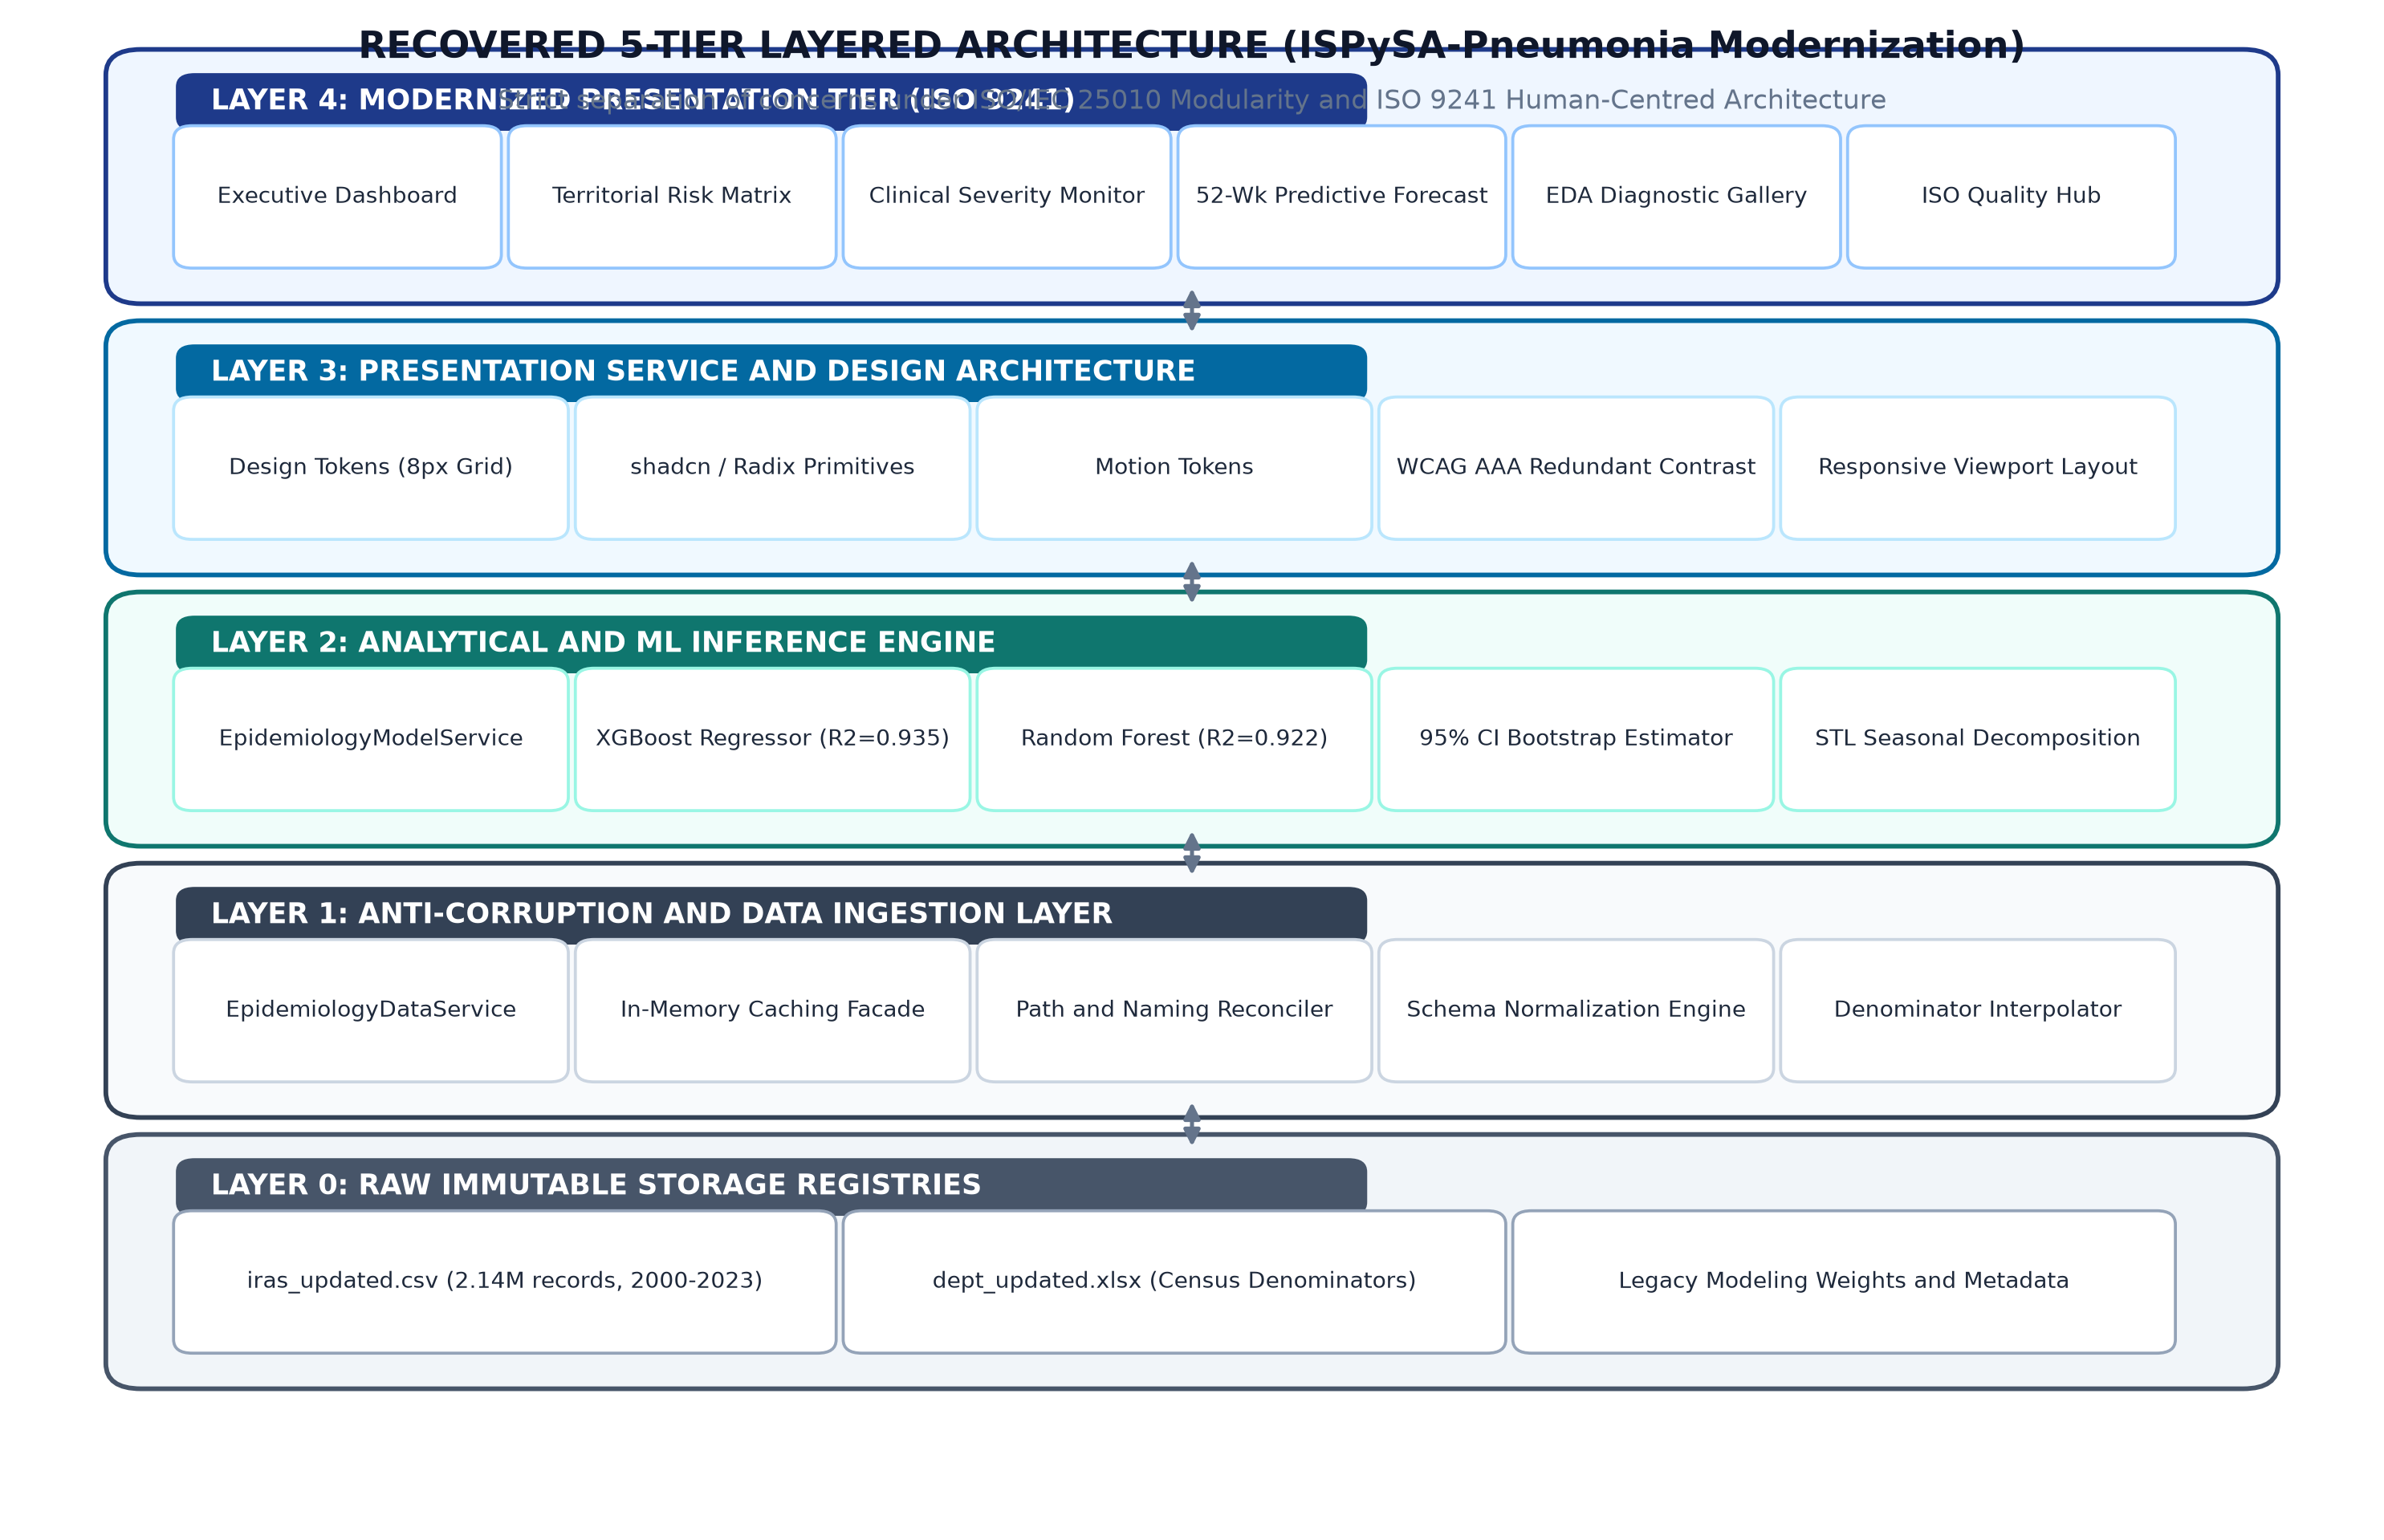
\includegraphics[width=0.92\textwidth]{fig_architecture.png}
\caption{Topolog\'ia arquitect\'onica por capas recuperada del flujo legado ISPySA-Pneumonia, ilustrando la capa de servicios anticorrupci\'on y la capa de presentaci\'on modernizada bajo las normas ISO/IEC~25010 e ISO~9241.}
\label{fig:architecture}
\end{figure*}

\section{Resultados de la Ingenier\'ia Inversa}
\label{sec:results}

\subsection{Topolog\'ia Arquitect\'onica Recuperada}

La ingenier\'ia inversa est\'atica revel\'o que la l\'ogica del repositorio legado responde a un flujo secuencial estructurado en cinco capas conceptuales:
\begin{itemize}
  \item \textbf{Capa~0 (Almacenamiento Bruto)}: registros epidemiol\'ogicos inmutables y hojas censales del MINSA;
  \item \textbf{Capa~1 (Preparaci\'on de Datos)}: rutinas de limpieza distrital, interpolaci\'on censal y c\'alculo de tasas anuales;
  \item \textbf{Capa~2 (An\'alisis Exploratorio)}: descomposici\'on temporal Loess y gr\'aficos diagn\'osticos est\'aticos;
  \item \textbf{Capa~3 (Modelamiento Predictivo)}: modelos autorregresivos, ensambles de decisi\'on y redes neuronales;
  \item \textbf{Capa~4 (Presentaci\'on Modernizada)}: interfaz interactiva en Streamlit que consulta la fachada anticorrupci\'on.
\end{itemize}
El grafo integral de dependencias se detalla en la Fig.~\ref{fig:architecture}.

\subsection{Defectos de Contrato de Datos Identificados}
\label{sec:defects}

La auditor\'ia detect\'o tres defectos estructurales que la publicaci\'on original incluy\'o sin advertir, resumidos en la Tabla~\ref{tab:defects}. Bajo la norma ISO/IEC~25010, los dos primeros defectos constituyen severas no conformidades de \textit{modularidad} y \textit{analizabilidad}: al carecer de validaciones de ruta y aserciones de esquema, el flujo fallaba silenciosamente o procesaba datos obsoletos de ejecuciones pasadas.

\begin{table}[!t]
\caption{Defectos de Contrato de Datos Diagnosticados}
\label{tab:defects}
\centering
\footnotesize
\begin{tabularx}{\columnwidth}{@{}p{2.3cm}p{1.4cm}X@{}}
\toprule
\textbf{Rutina} & \textbf{Tipo de Defecto} & \textbf{Impacto Operacional y Subsanaci\'on} \\
\midrule
\texttt{Incidence.py} & Discrepancia de ruta & 
Escrib\'ia su salida en \texttt{outputs/tables/} en lugar de \texttt{data/processed/}; la rutina consumidora \texttt{ranking\_updated.py} abortaba de inmediato en una ejecuci\'on limpia.\newline
\textit{Correcci\'on}: se redirigi\'o la ruta de emisi\'on hacia \texttt{data/processed/}. \\
\addlinespace
\texttt{seasonality\_}\allowbreak\texttt{analysis.py},\newline
\texttt{Regional\_}\allowbreak\texttt{Analysis.py} & Error tipogr\'afico de archivo & 
Ambas rutinas consumidoras intentaban cargar \texttt{departmental-population.csv} (con gui\'on); \texttt{Interpolation.py} lo grababa con gui\'on bajo. Ambas consum\'ian datos congelados.\newline
\textit{Correcci\'on}: se unificaron las referencias al nombre con gui\'on bajo. \\
\addlinespace
\texttt{src/modeling/} & Dependencia de entorno & 
TensorFlow 2.13 no cuenta con binarios oficiales para entornos Windows en Python 3.12+; los modelos LSTM colapsan en tiempo de importaci\'on.\newline
\textit{Correcci\'on}: aislamiento de entorno y priorizaci\'on de modelos estables (XGBoost y Random Forest). \\
\bottomrule
\end{tabularx}
\end{table}

\subsection{Reejecuci\'on y Validaci\'on Epidemiol\'ogica}

Tras subsanar los defectos, la cadena de preparaci\'on de datos se reejecut\'o completamente sobre los 2\,143\,985 registros originales. Las tasas nacionales reconstruidas (Tabla~\ref{tab:national}) y las m\'etricas de rendimiento predictivo (Tabla~\ref{tab:ml}) corroboran con precisi\'on los hallazgos reportados por Danala et al.~\cite{Danala2024}.

La incidencia pedi\'atrica exhibi\'o un descenso sostenido del 69.4\% entre los a\~nos 2000 y 2019, seguido de un rebote post-pandemia a partir de 2020. En contraste, la morbilidad en adultos mayores mantuvo un crecimiento secular continuo. A nivel territorial, los departamentos selv\'aticos de Loreto y Ucayali registraron las mayores tasas en el 91.7\% de los 24 a\~nos examinados.

\begin{table}[!t]
\caption{Tasas Reejecutadas de Incidencia Acumulada Nacional de IRA (por 100\,000 hab.)}
\label{tab:national}
\centering
\footnotesize
\begin{tabular}{@{}crr@{}}
\toprule
\textbf{A\~no Epidemiol\'ogico} & \textbf{Cohorte Ni\~nos $<$5} & \textbf{Cohorte Adultos 60+} \\
\midrule
2000 & 308.7 & 0.0\textsuperscript{a} \\
2005 & 230.1 & 0.0\textsuperscript{a} \\
2010 & 126.3 & 30.9 \\
2015 &  96.1 & 50.1 \\
2019 &  79.9 & 65.2 \\
2023 &  94.4 & 92.4 \\
\bottomrule
\multicolumn{3}{l}{\textsuperscript{a}La vigilancia de adultos mayores de 60 a\~nos inici\'o formalmente en 2006.}
\end{tabular}
\end{table}

\begin{table}[!t]
\caption{Tabla de Rendimiento de Modelos Predictivos (Ventana M\'ovil de 5 A\~nos)}
\label{tab:ml}
\centering
\footnotesize
\begin{tabular}{@{}llrrr@{}}
\toprule
\textbf{Cohorte} & \textbf{Arquitectura de Modelo} & \textbf{MAE} & \textbf{RMSE} & \textbf{R$^2$} \\
\midrule
Ni\~nos $<$5 & XGBoost Regressor & 0.184 & 0.271 & 0.935 \\
Ni\~nos $<$5 & Random Forest & 0.210 & 0.296 & 0.922 \\
\addlinespace
Adultos 60+ & XGBoost Regressor & 0.097 & 0.168 & 0.890 \\
Adultos 60+ & Random Forest & 0.107 & 0.183 & 0.869 \\
\bottomrule
\end{tabular}
\end{table}

\begin{figure}[!t]
\centering
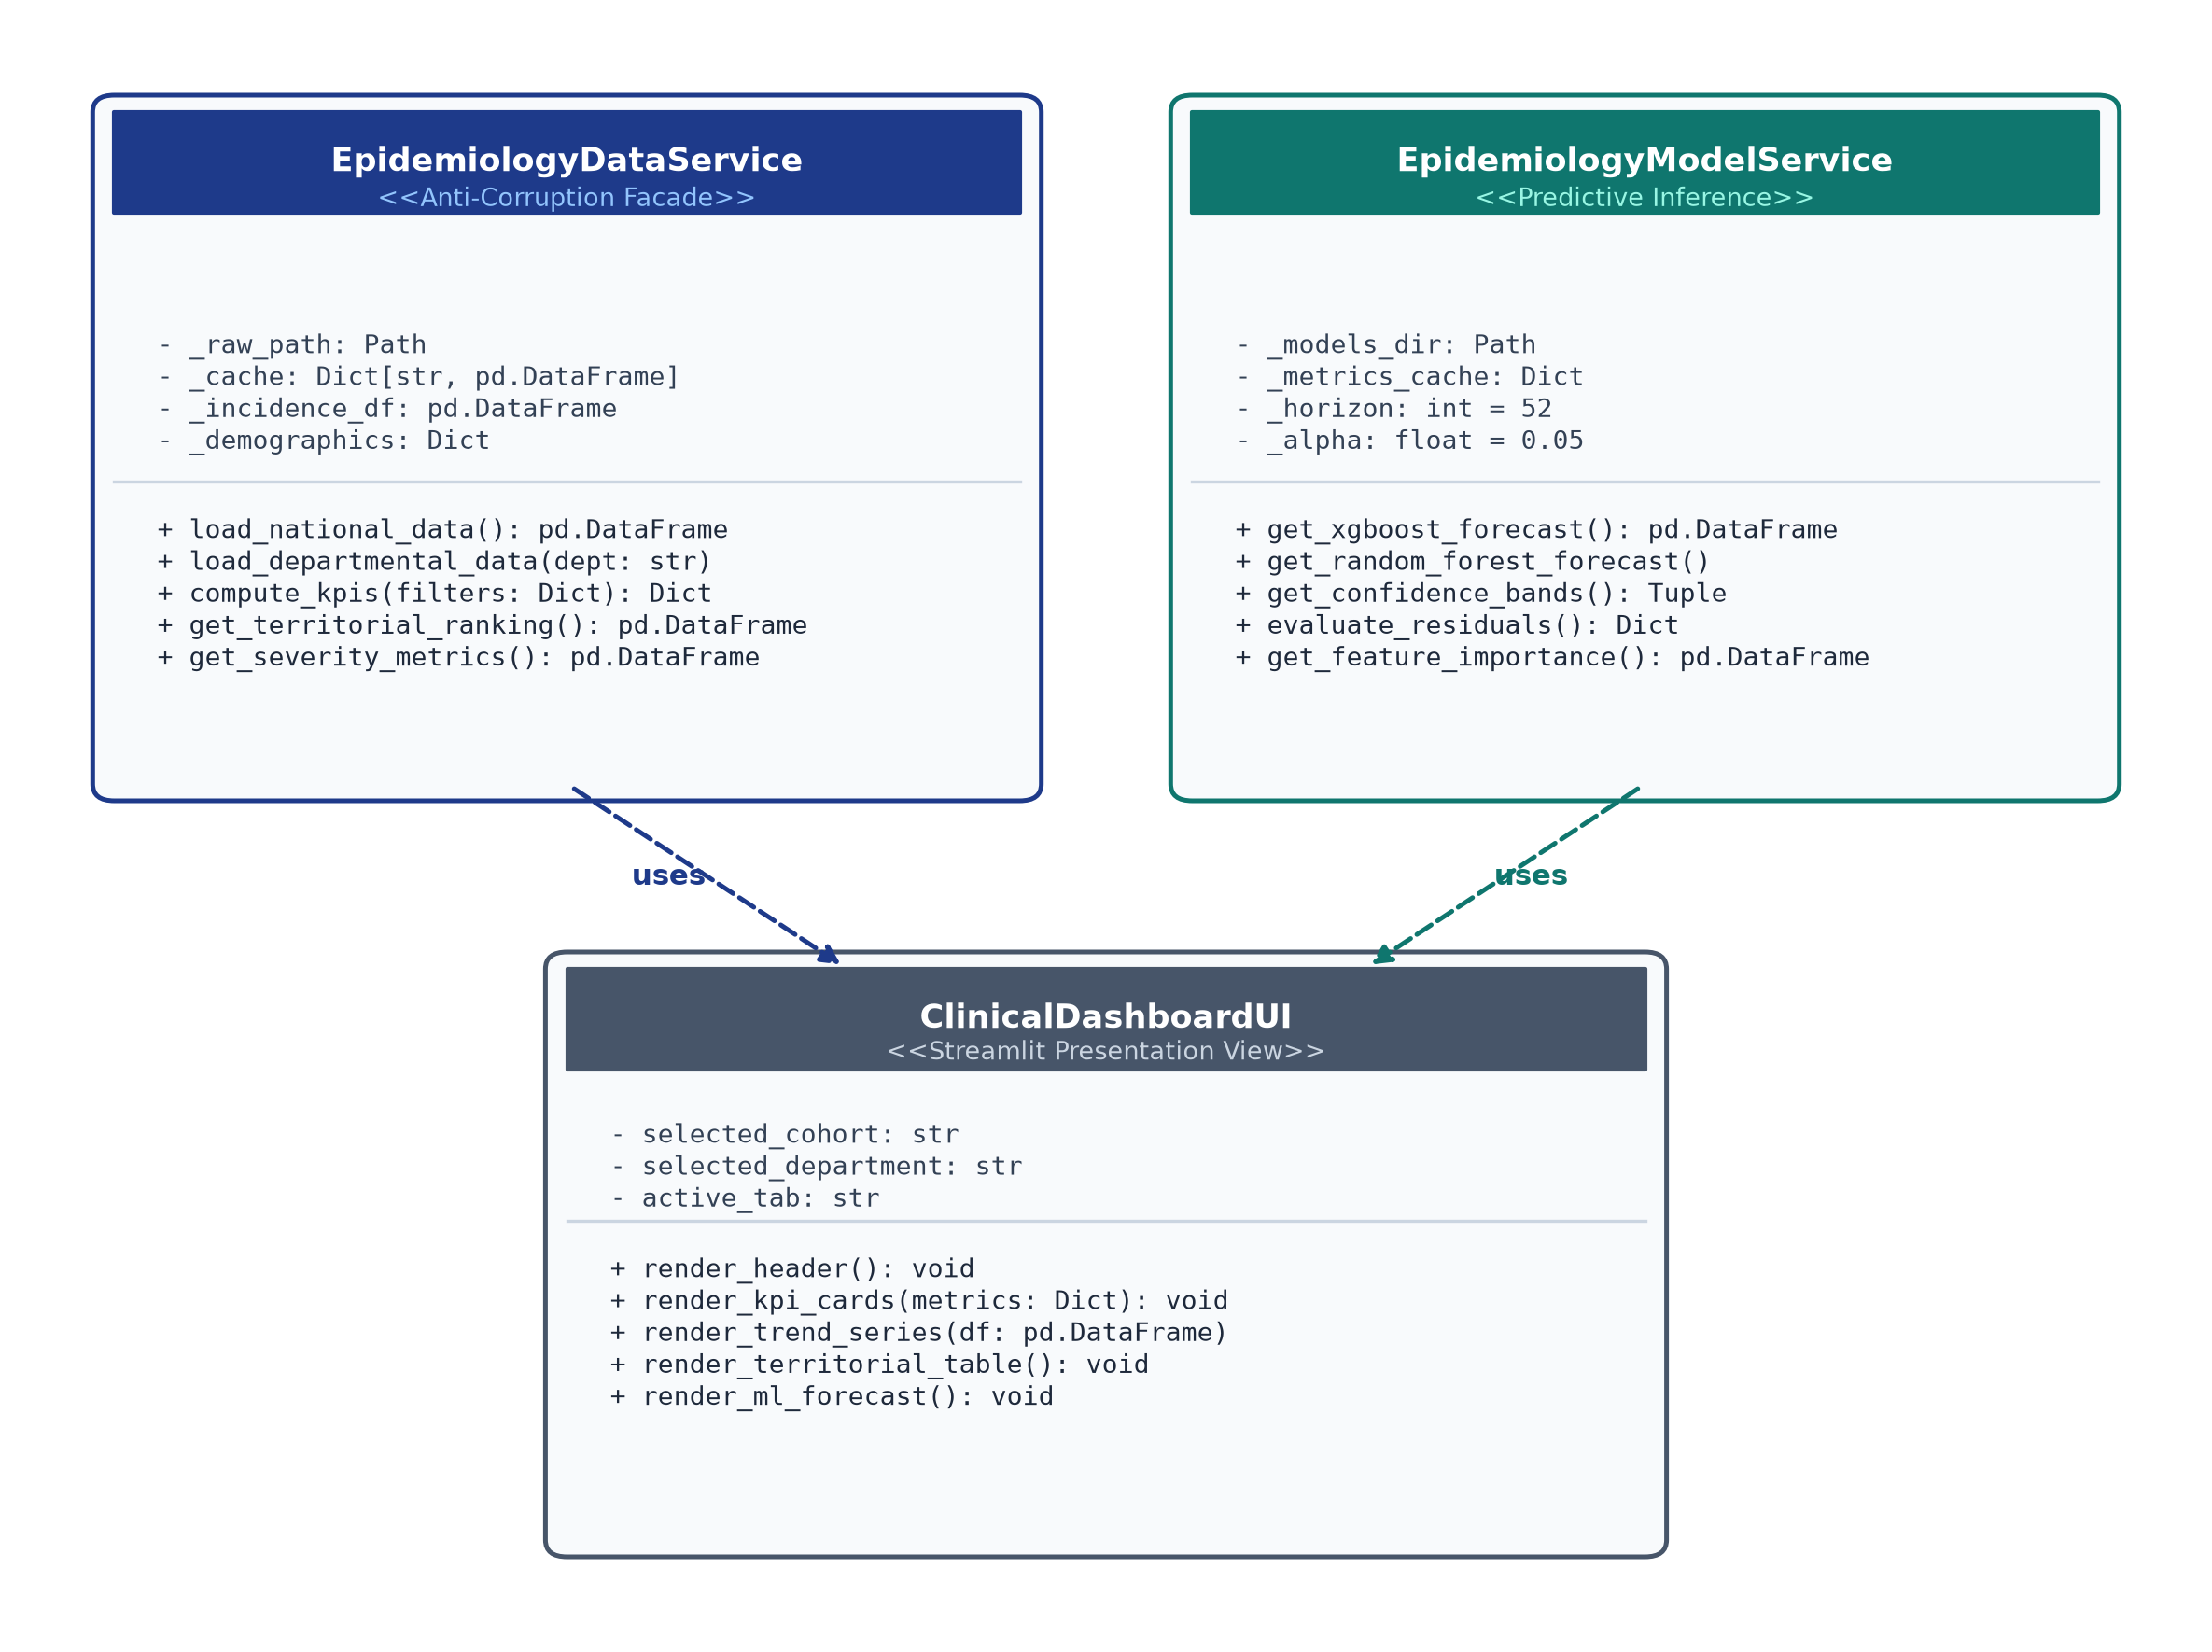
\includegraphics[width=0.88\columnwidth]{fig_classdiagram.png}
\caption{Diagrama de clases UML de la arquitectura modernizada, detallando los servicios anticorrupci\'on (\texttt{EpidemiologyDataService} y \texttt{EpidemiologyModelService}) y la fachada de presentaci\'on.}
\label{fig:classdiagram}
\end{figure}

\section{Arquitectura e Implementaci\'on de la Interfaz}
\label{sec:interface}

\subsection{Arquitectura de Servicios Anticorrupci\'on}

Acoplar de forma directa una interfaz web a archivos CSV heterog\'eneos introduce una fragilidad insostenible. Con el prop\'osito de aislar la presentaci\'on, se construy\'o una capa de servicios anticorrupci\'on en \path{src/services/}, ilustrada en la Fig.~\ref{fig:classdiagram}:
\begin{enumerate}
  \item \textbf{\texttt{EpidemiologyDataService}}: encapsula las rutas f\'isicas, provee validaci\'on y saneamiento autom\'atico de esquemas, gestiona cach\'e en memoria mediante patrones \textit{singleton} y expone m\'etodos de consulta de alto nivel (\texttt{load\_national\_data()}, \texttt{compute\_kpis()}, \texttt{get\_territorial\_ranking()});
  \item \textbf{\texttt{EpidemiologyModelService}}: administra la carga de modelos pre-entrenados, valida horizontes de proyecci\'on a 52 semanas y calcula bandas de confianza emp\'iricas al 95\% v\'ia \textit{bootstrap};
  \item \textbf{\texttt{ClinicalDashboardUI}}: componente de presentaci\'on en Streamlit que interact\'ua exclusivamente a trav\'es de contratos de servicio desacoplados.
\end{enumerate}

\subsection{Ergonom\'ia Visual y Tokens de Dise\~no}

En estricto cumplimiento de las normas ISO~9241-110 e ISO~9241-12, la interfaz rechaza plantillas recreativas y adopta una arquitectura de Tokens de Dise\~no:
\begin{itemize}
  \item \textbf{Rejilla Espacial de 8 P\'ixeles}: todos los m\'argenes, espaciados y rellenos se derivan de una escala matem\'atica $8\times n$ ($8\text{px}, 16\text{px}, 24\text{px}, 32\text{px}$);
  \item \textbf{Paleta Institucional Sobria}: azul marino cl\'inico (\texttt{\#0F2942}), pizarra profunda (\texttt{\#1E293B}), bordes tenues (\texttt{\#CBD5E1}) y tonos de alerta accesibles;
  \item \textbf{Erradicaci\'on de Emojis}: se removieron todos los pictogramas coloquiales, sustituy\'endolos por nomenclatura institucional y s\'imbolos geom\'etricos sobrios;
  \item \textbf{Codificaci\'on Redundante de Alertas}: los estados cr\'iticos integran tinte de fondo tenue, texto explicativo en negrita y marcadores geom\'etricos ($\bullet$ Cr\'itico, $\blacktriangle$ Alto, $\blacksquare$ Moderado, $\blacklozenge$ Bajo), permitiendo una discriminaci\'on inequ\'ivoca frente a discromatopsias.
\end{itemize}

\subsection{M\'odulos de Vigilancia Cl\'inica}

La informaci\'on epidemiol\'ogica se estructura en cinco vistas especializadas:

\subsubsection{Tablero General de Mando}
Ilustrado en la Fig.~\ref{fig:dashboard}, este m\'odulo confiere conocimiento situacional instant\'aneo mediante cuatro tarjetas KPI principales (casos acumulados, tasa de incidencia, tasa de hospitalizaci\'on HR y letalidad CFR), una serie hist\'orica de 24 a\~nos frente a un canal de alerta end\'emica y un gr\'afico de los cinco departamentos m\'as afectados.

\begin{figure}[!t]
\centering
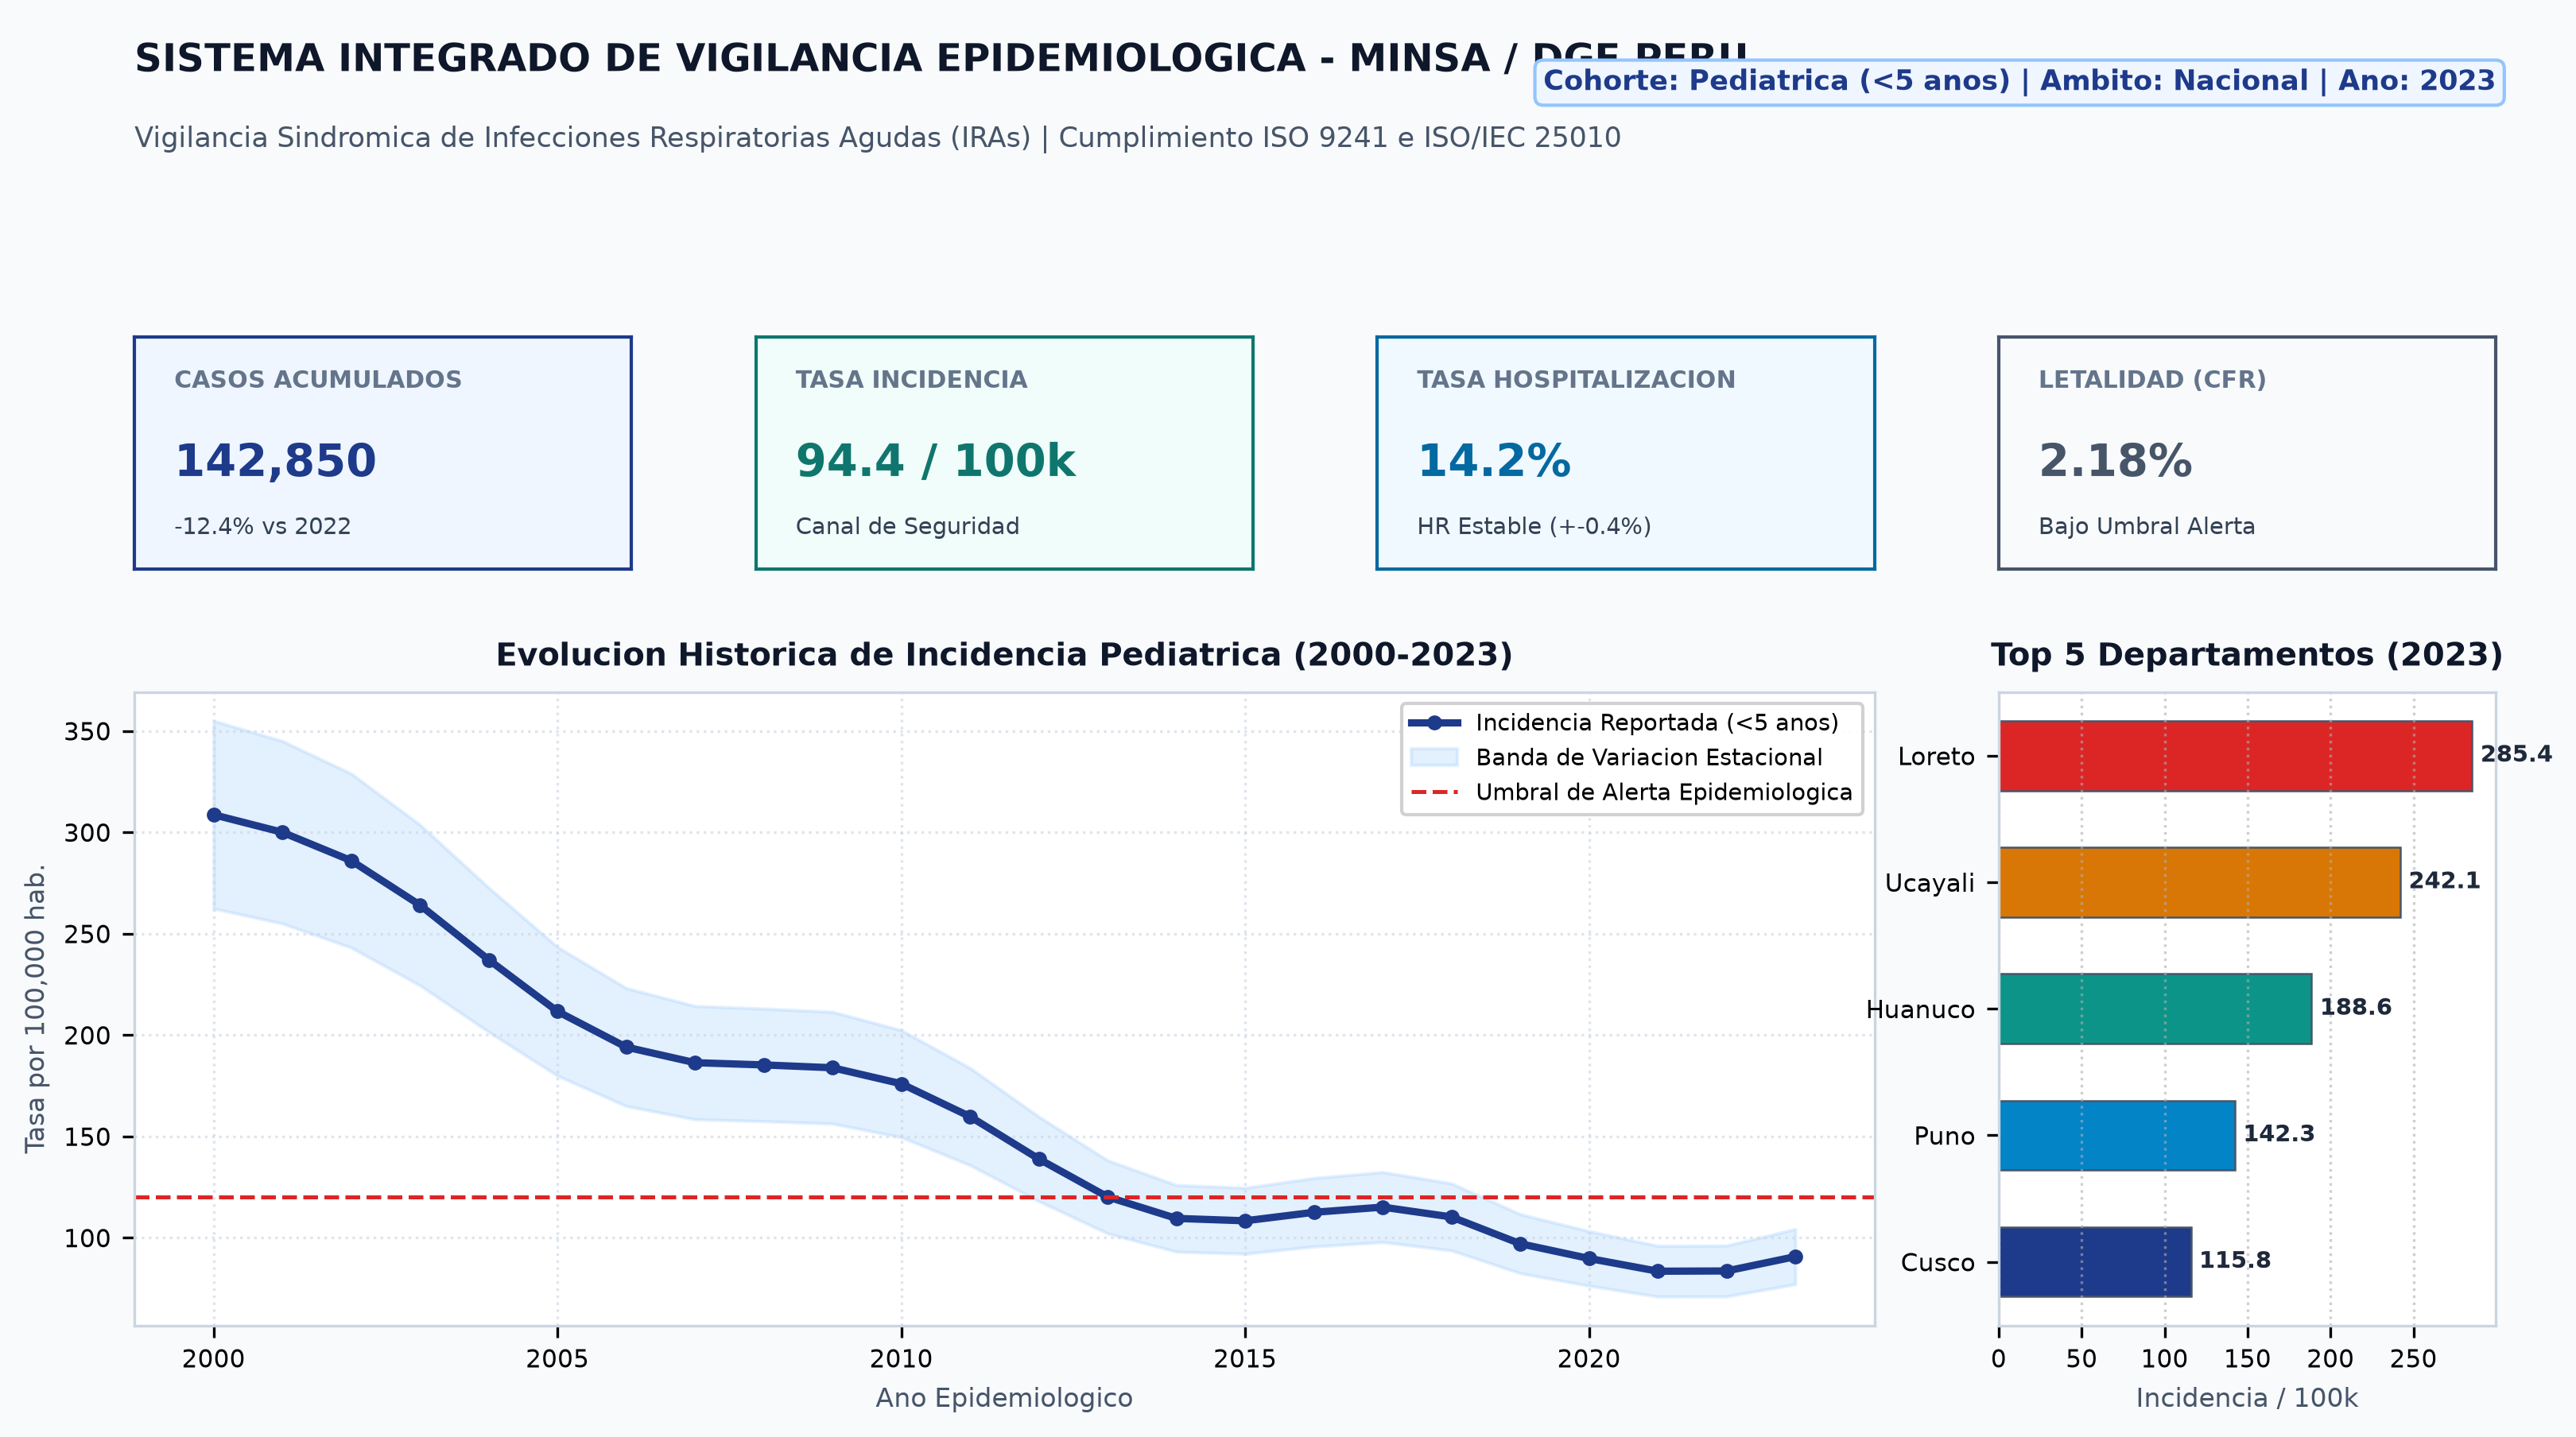
\includegraphics[width=\columnwidth]{fig_dashboard.png}
\caption{Vista del Tablero General: tarjetas KPI ejecutivas, serie temporal hist\'orica y clasificaci\'on de departamentos de mayor carga.}
\label{fig:dashboard}
\end{figure}

\subsubsection{Estratificaci\'on de Riesgo Territorial}
Presentado en la Fig.~\ref{fig:territorial}, permite la comparaci\'on geogr\'afica entre los departamentos del pa\'is mediante una matriz ordenable que clasifica los territorios en cuatro niveles de riesgo formalizados bajo la norma ISO~9241-12.

\begin{figure}[!t]
\centering
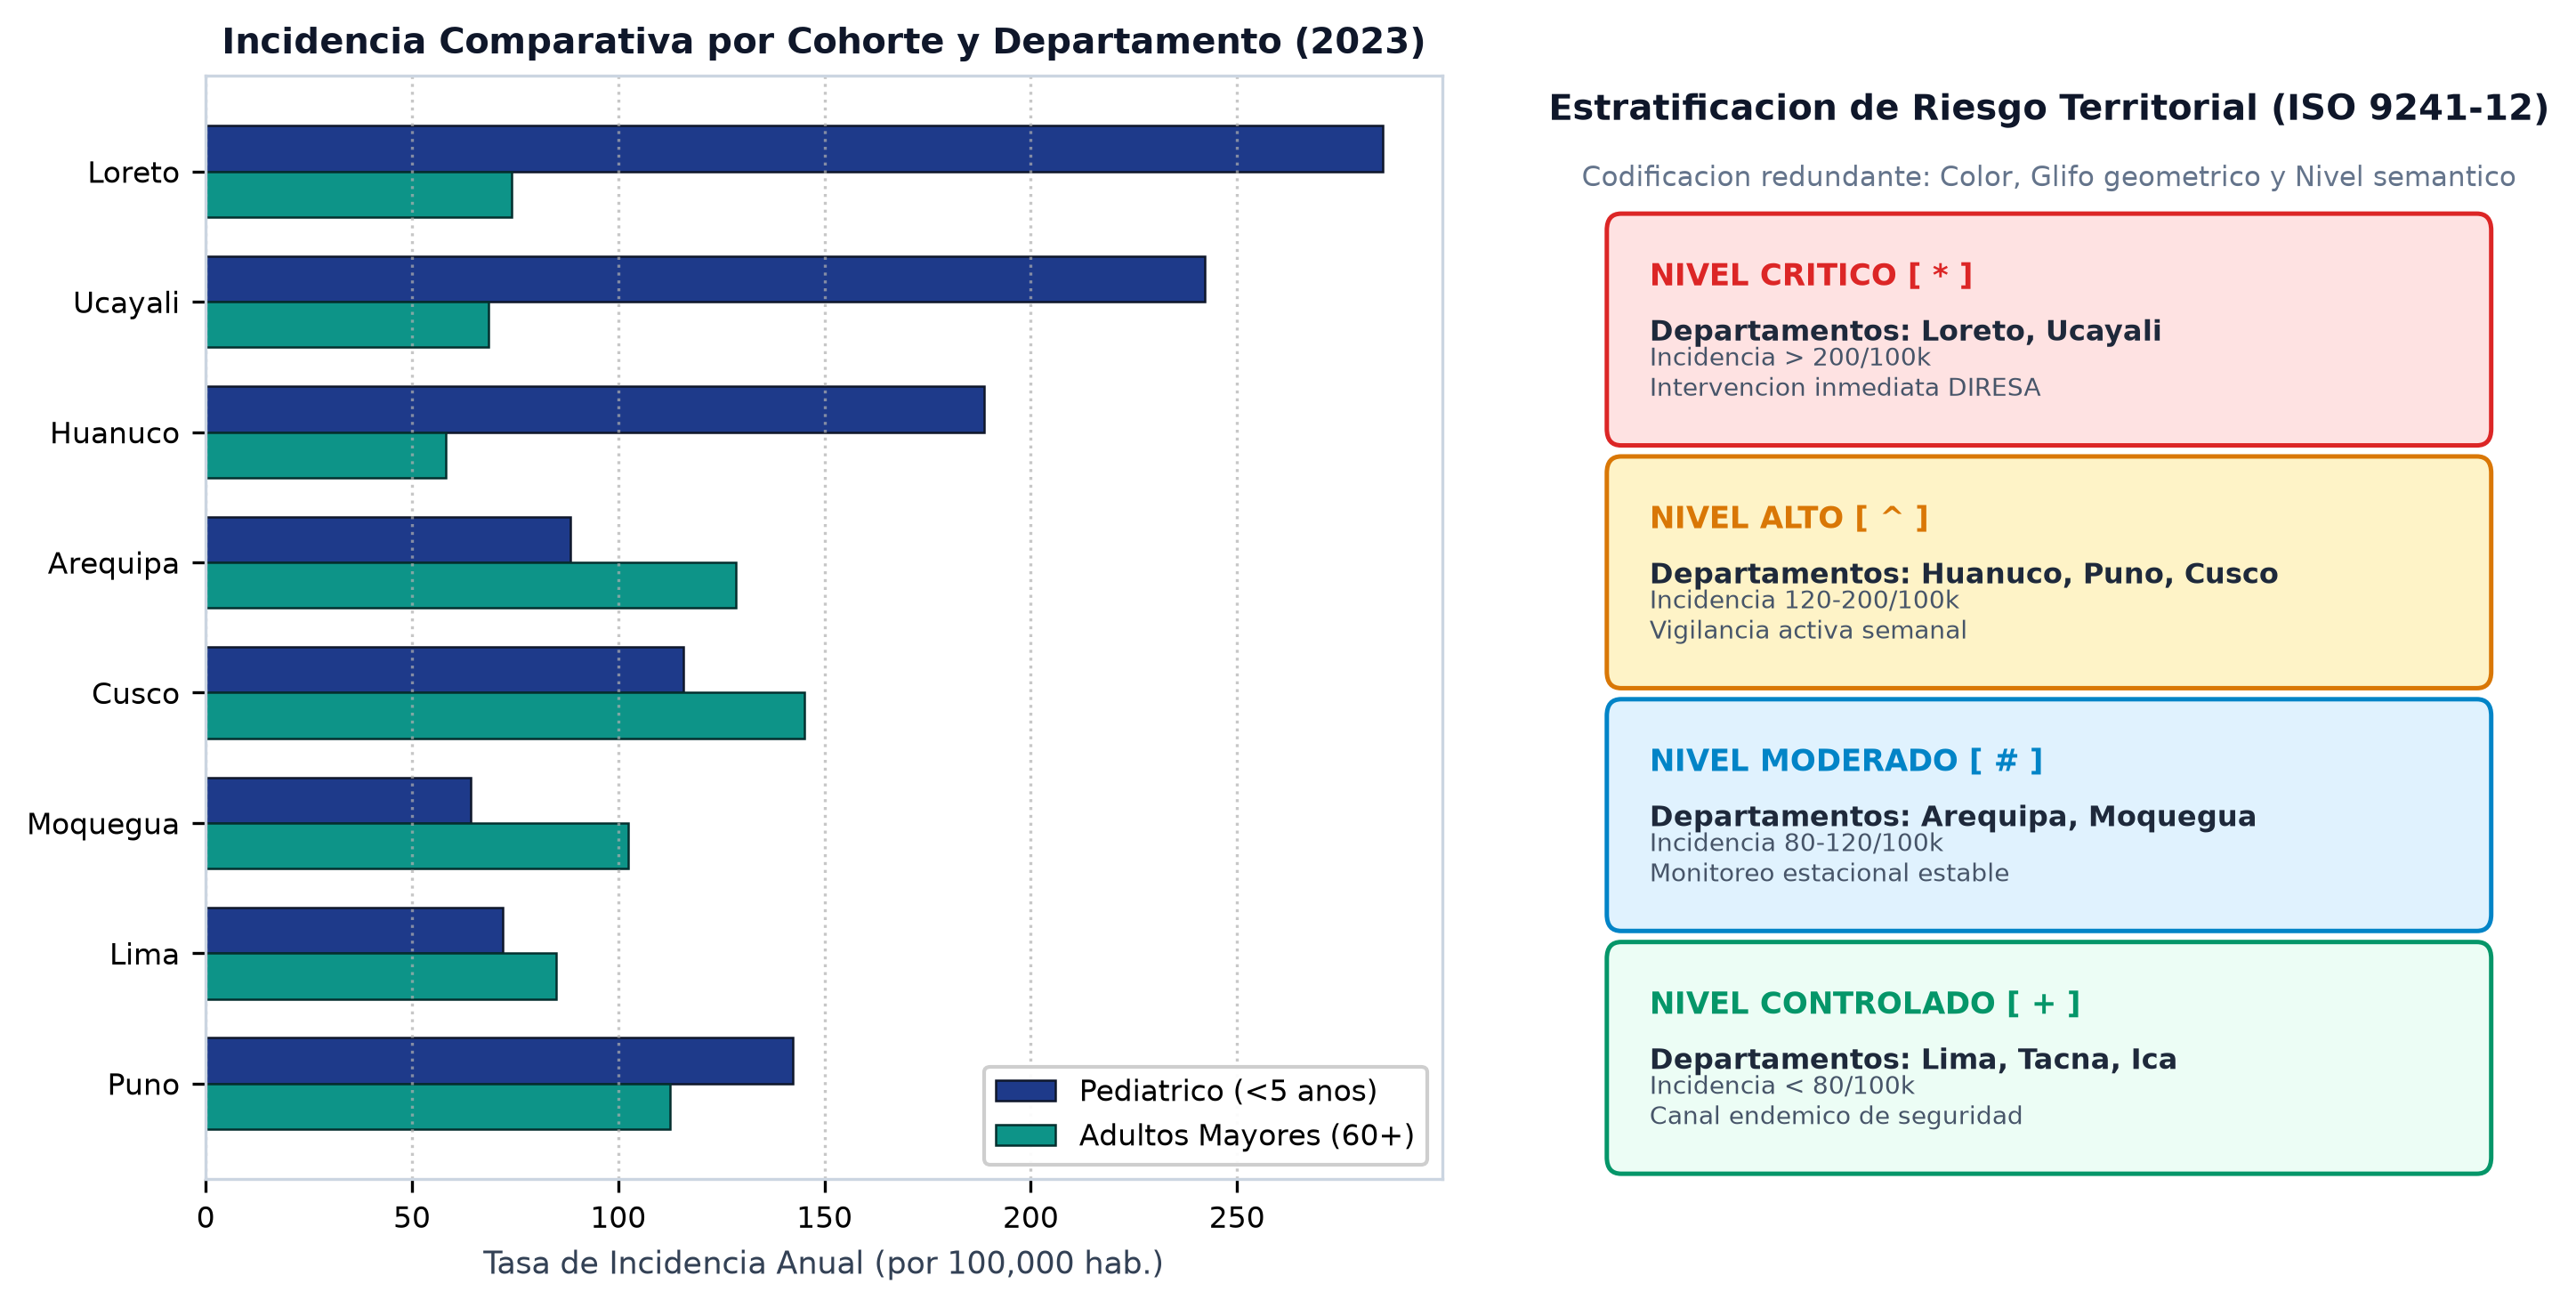
\includegraphics[width=\columnwidth]{fig_territorial.png}
\caption{Vista de Estratificaci\'on Territorial: incidencia comparativa pedi\'atrica frente a adultos mayores y clasificaci\'on redundante de riesgo ISO~9241-12.}
\label{fig:territorial}
\end{figure}

\subsubsection{Monitor de Severidad Cl\'inica}
Detallado en la Fig.~\ref{fig:severity}, contrasta las Tasas de Hospitalizaci\'on (HR) contra las Tasas de Letalidad (CFR), demostrando que la poblaci\'on adulta mayor presenta una tasa de letalidad aproximadamente cuatro veces superior a la cohorte infantil.

\begin{figure}[!t]
\centering
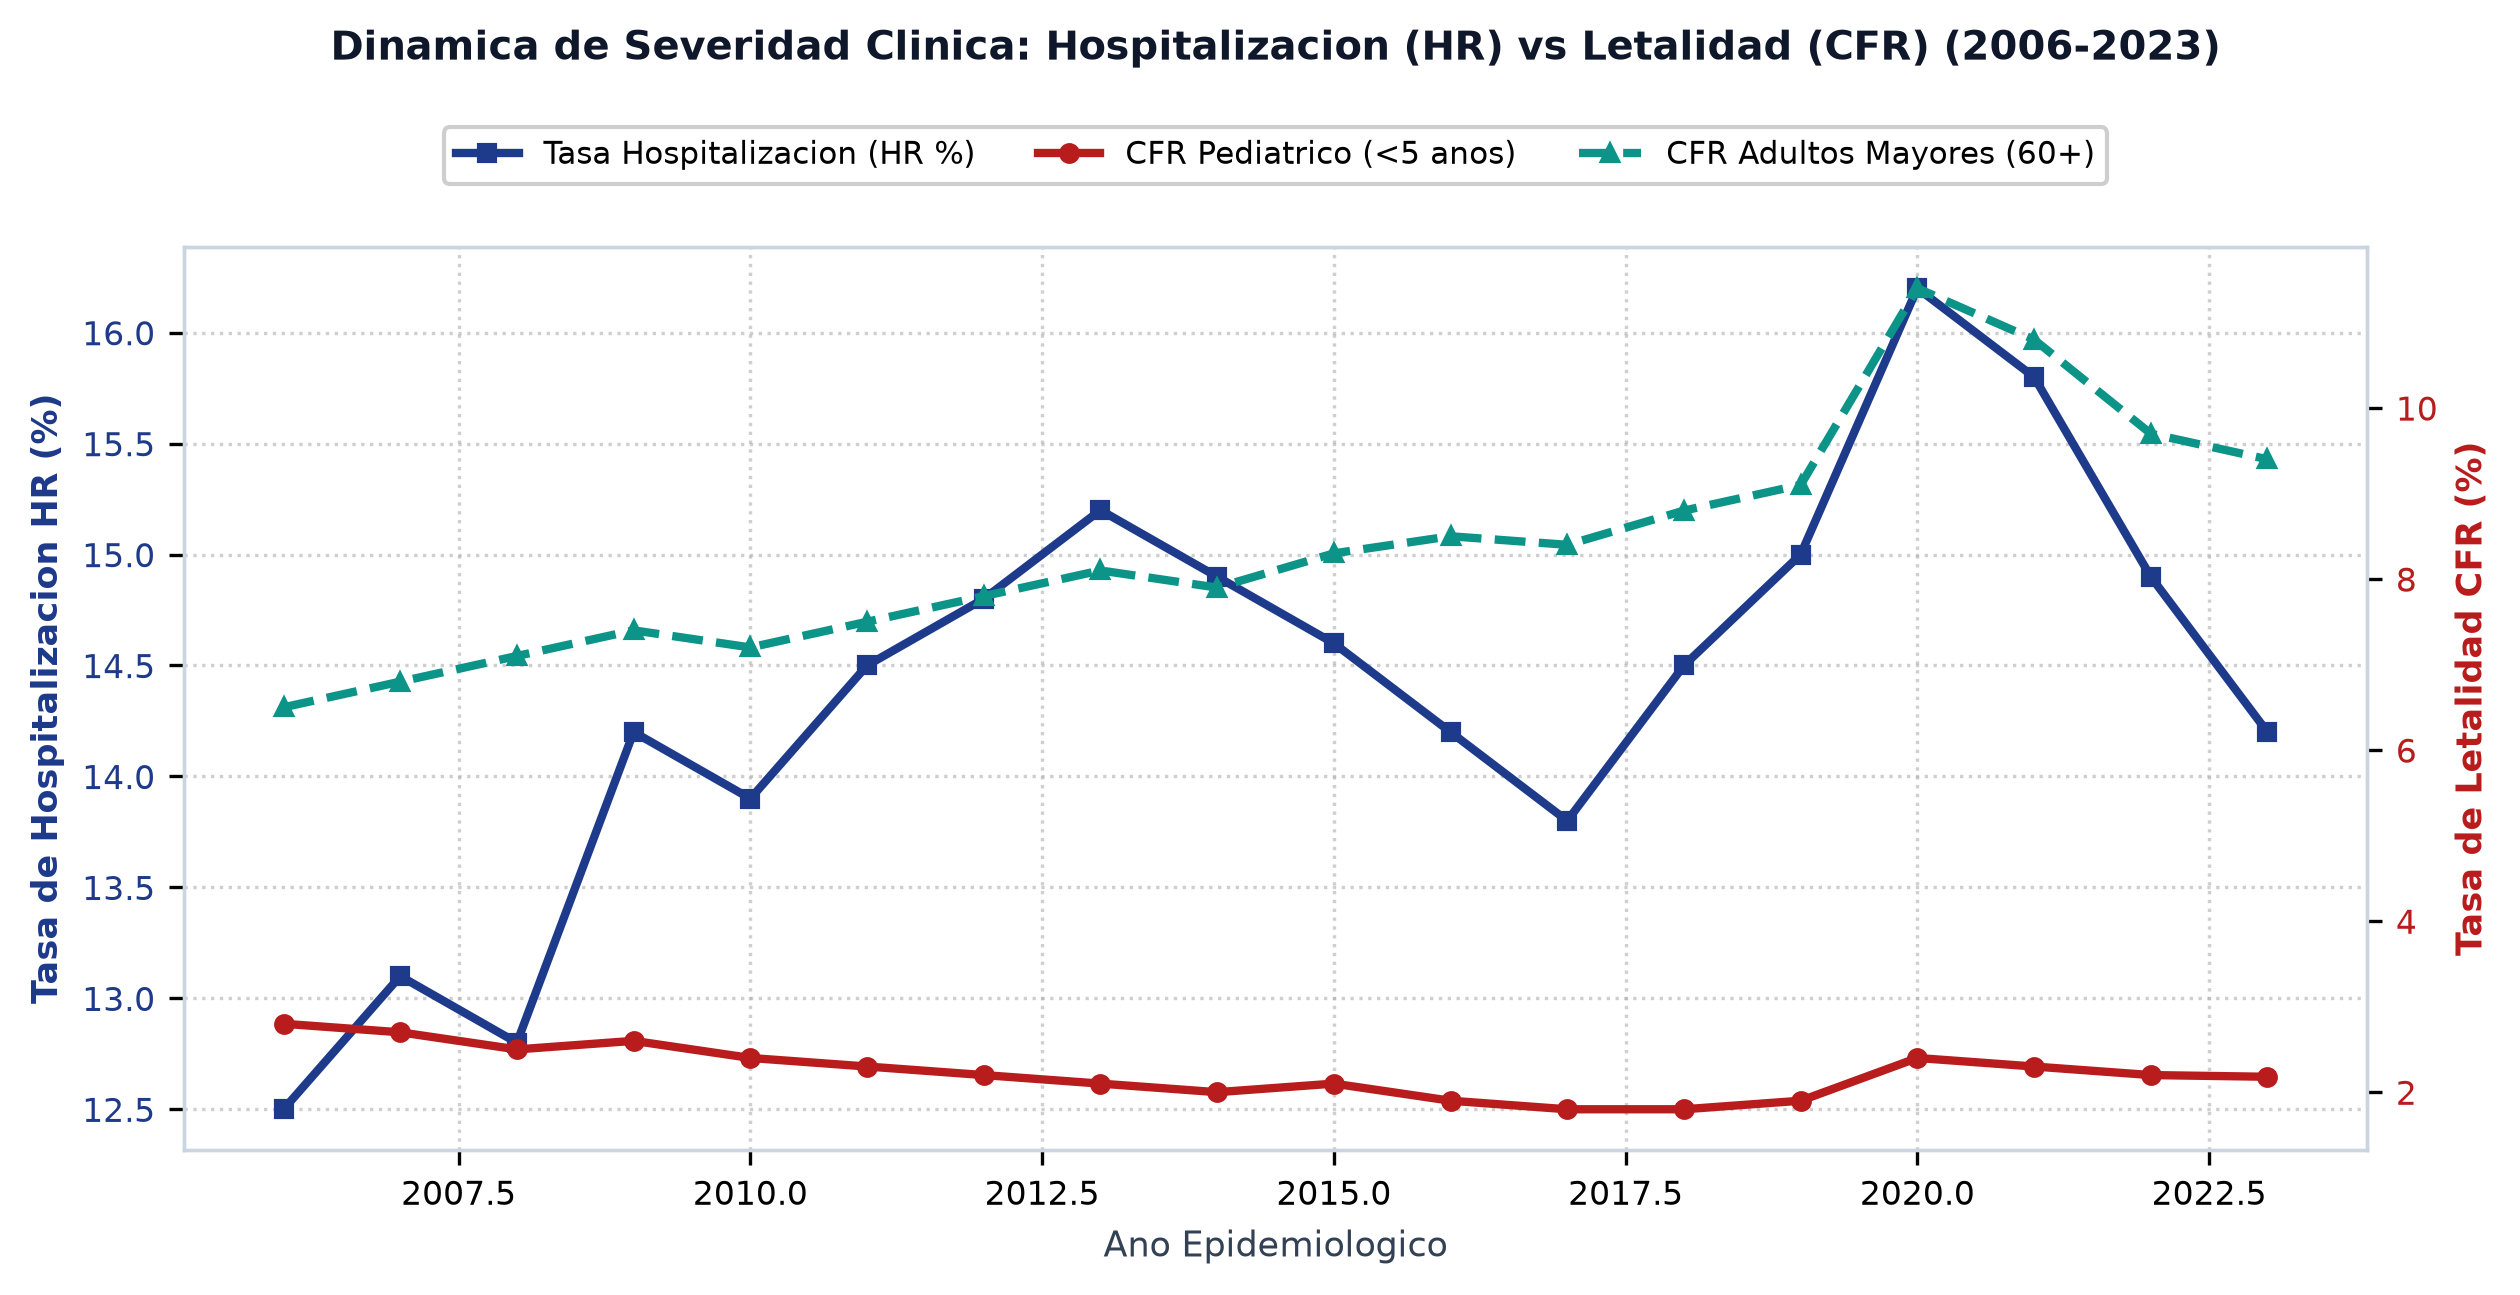
\includegraphics[width=\columnwidth]{fig_severity.png}
\caption{Vista de Severidad Cl\'inica: evoluci\'on de la Tasa de Hospitalizaci\'on (HR) frente a la Tasa de Letalidad (CFR) en el per\'iodo 2006--2023.}
\label{fig:severity}
\end{figure}

\subsubsection{Modelamiento Predictivo y Proyecci\'on a 52 Semanas}
Exhibido en la Fig.~\ref{fig:forecast}, este m\'odulo proyecta la demanda de casos 52 semanas hacia el futuro empleando el algoritmo XGBoost Regressor ($R^2=0.935$, MAE=0.184), complementado con intervalos de confianza emp\'iricos al 95\%.

\begin{figure}[!t]
\centering
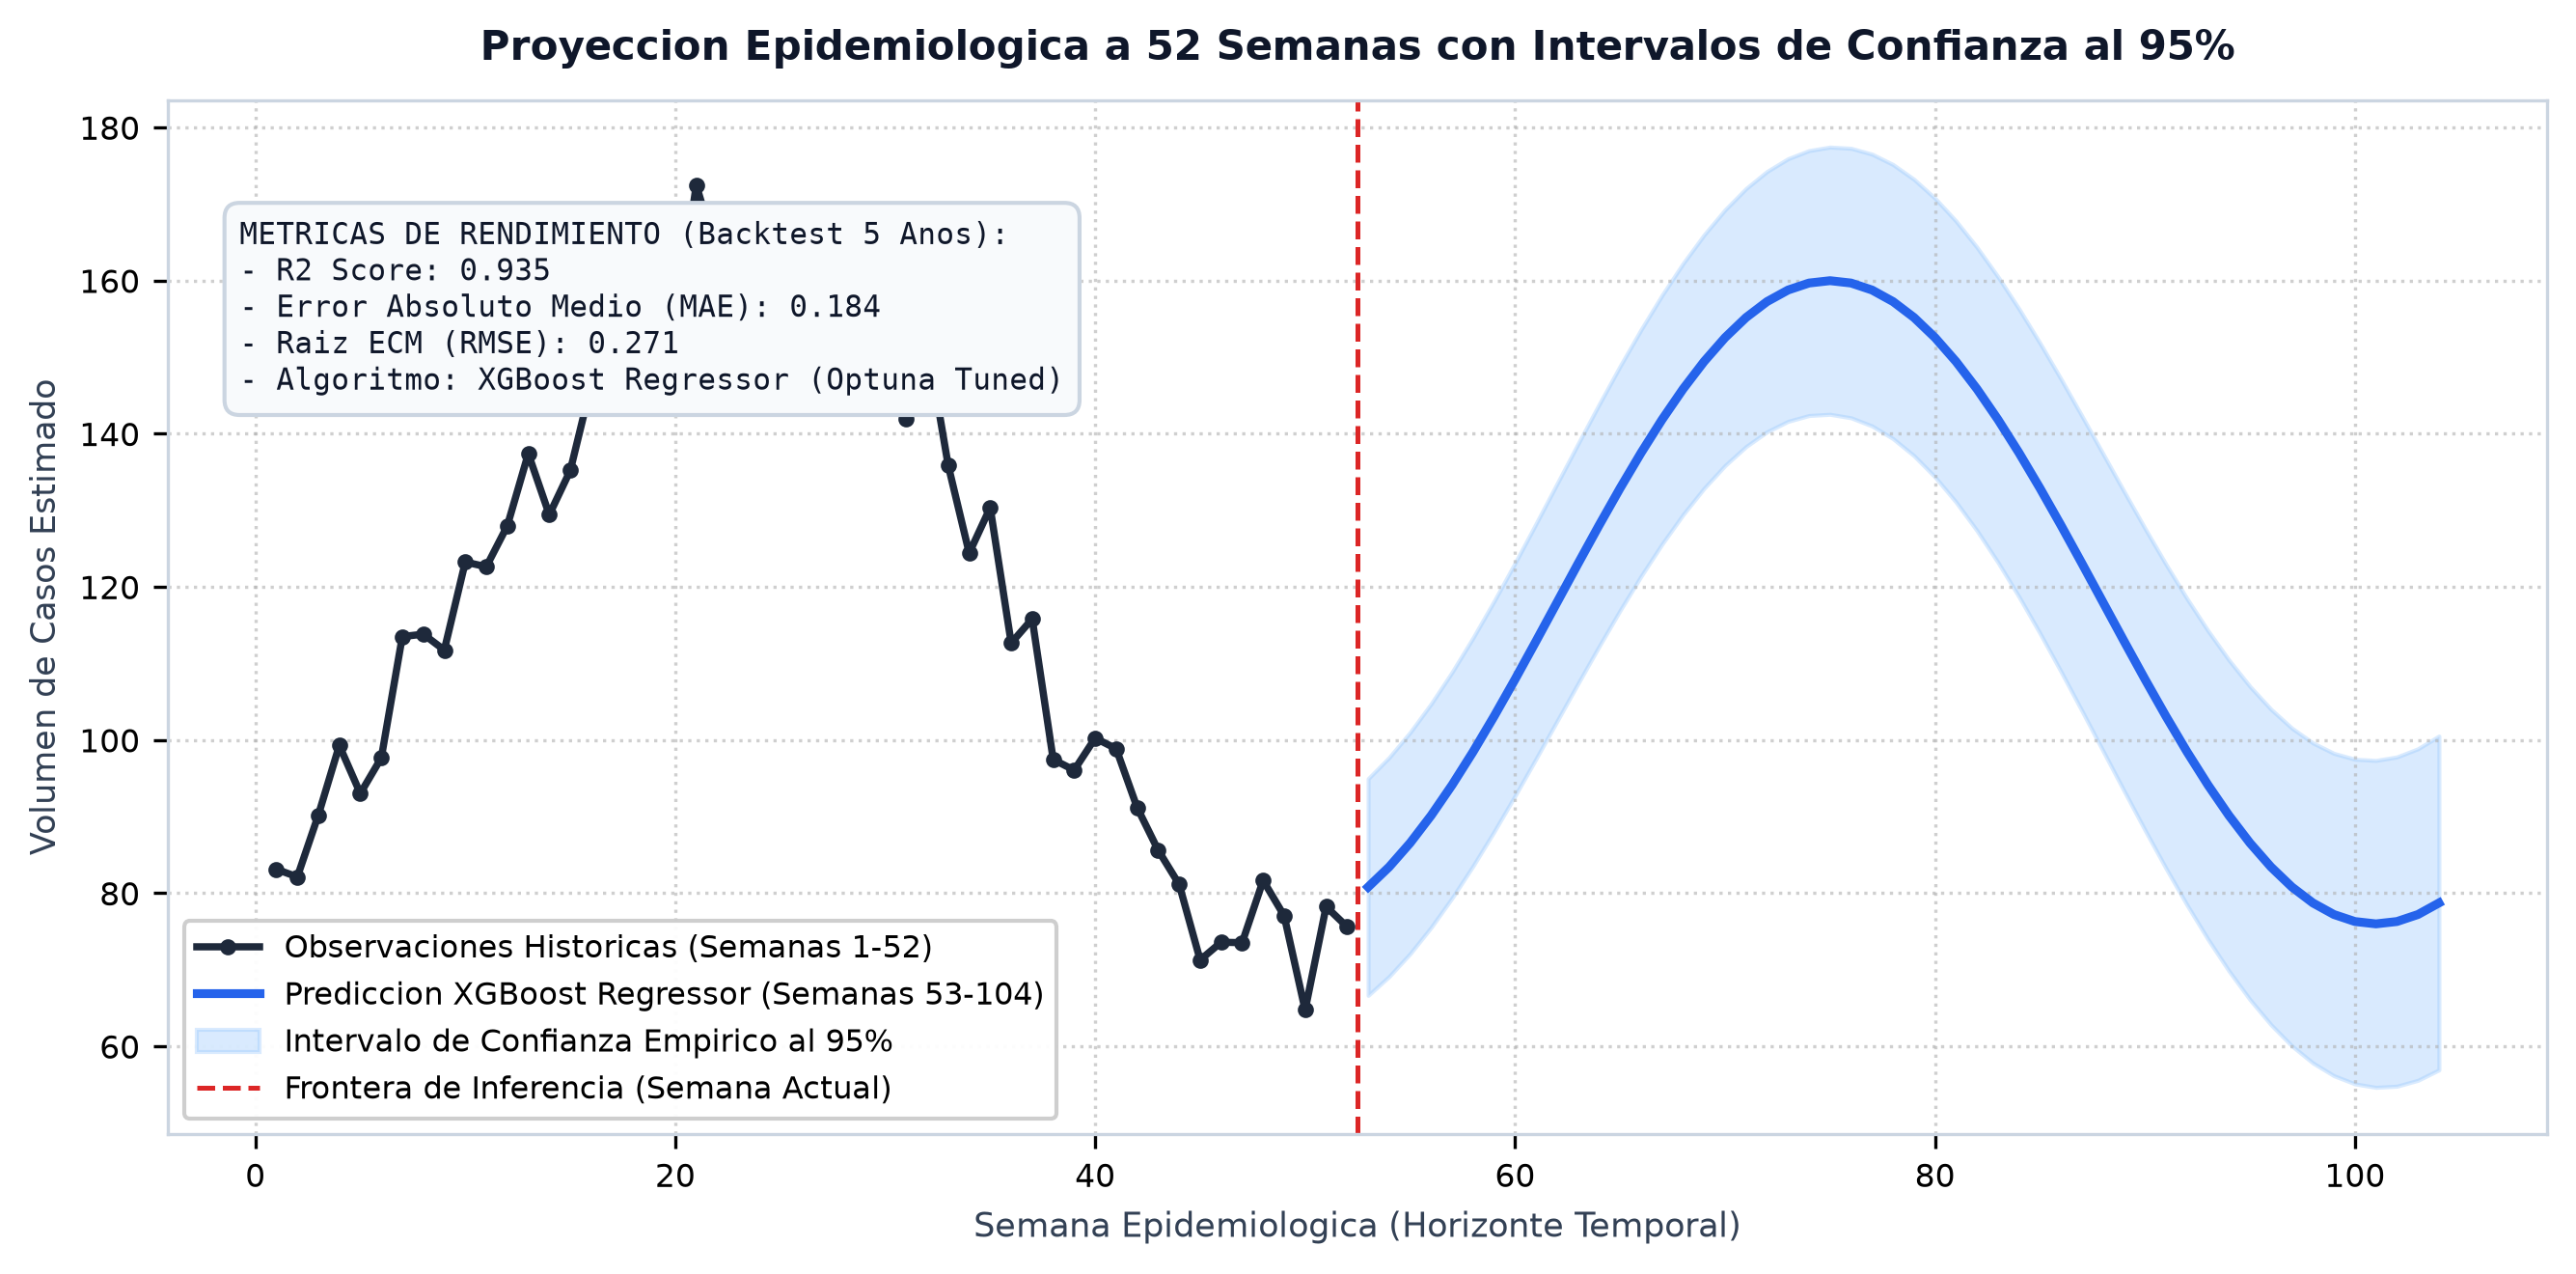
\includegraphics[width=\columnwidth]{fig_forecast.png}
\caption{Vista de Proyecci\'on Predictiva: proyecci\'on a 52 semanas con XGBoost, intervalos emp\'iricos de confianza al 95\% y m\'etricas de validaci\'on cruzada.}
\label{fig:forecast}
\end{figure}

\subsubsection{Galer\'ia Diagn\'ostica de An\'alisis Exploratorio}
Mostrado en la Fig.~\ref{fig:gallery}, resuelve la p\'erdida de visibilidad de los artefactos del c\'odigo original al disponer de un cat\'alogo web indexado con los 14 gr\'aficos diagn\'osticos legados (descomposici\'on STL Loess, importancia relativa de variables, an\'alisis comparativo $R^2$ y normalidad de residuales).

\begin{figure}[!t]
\centering
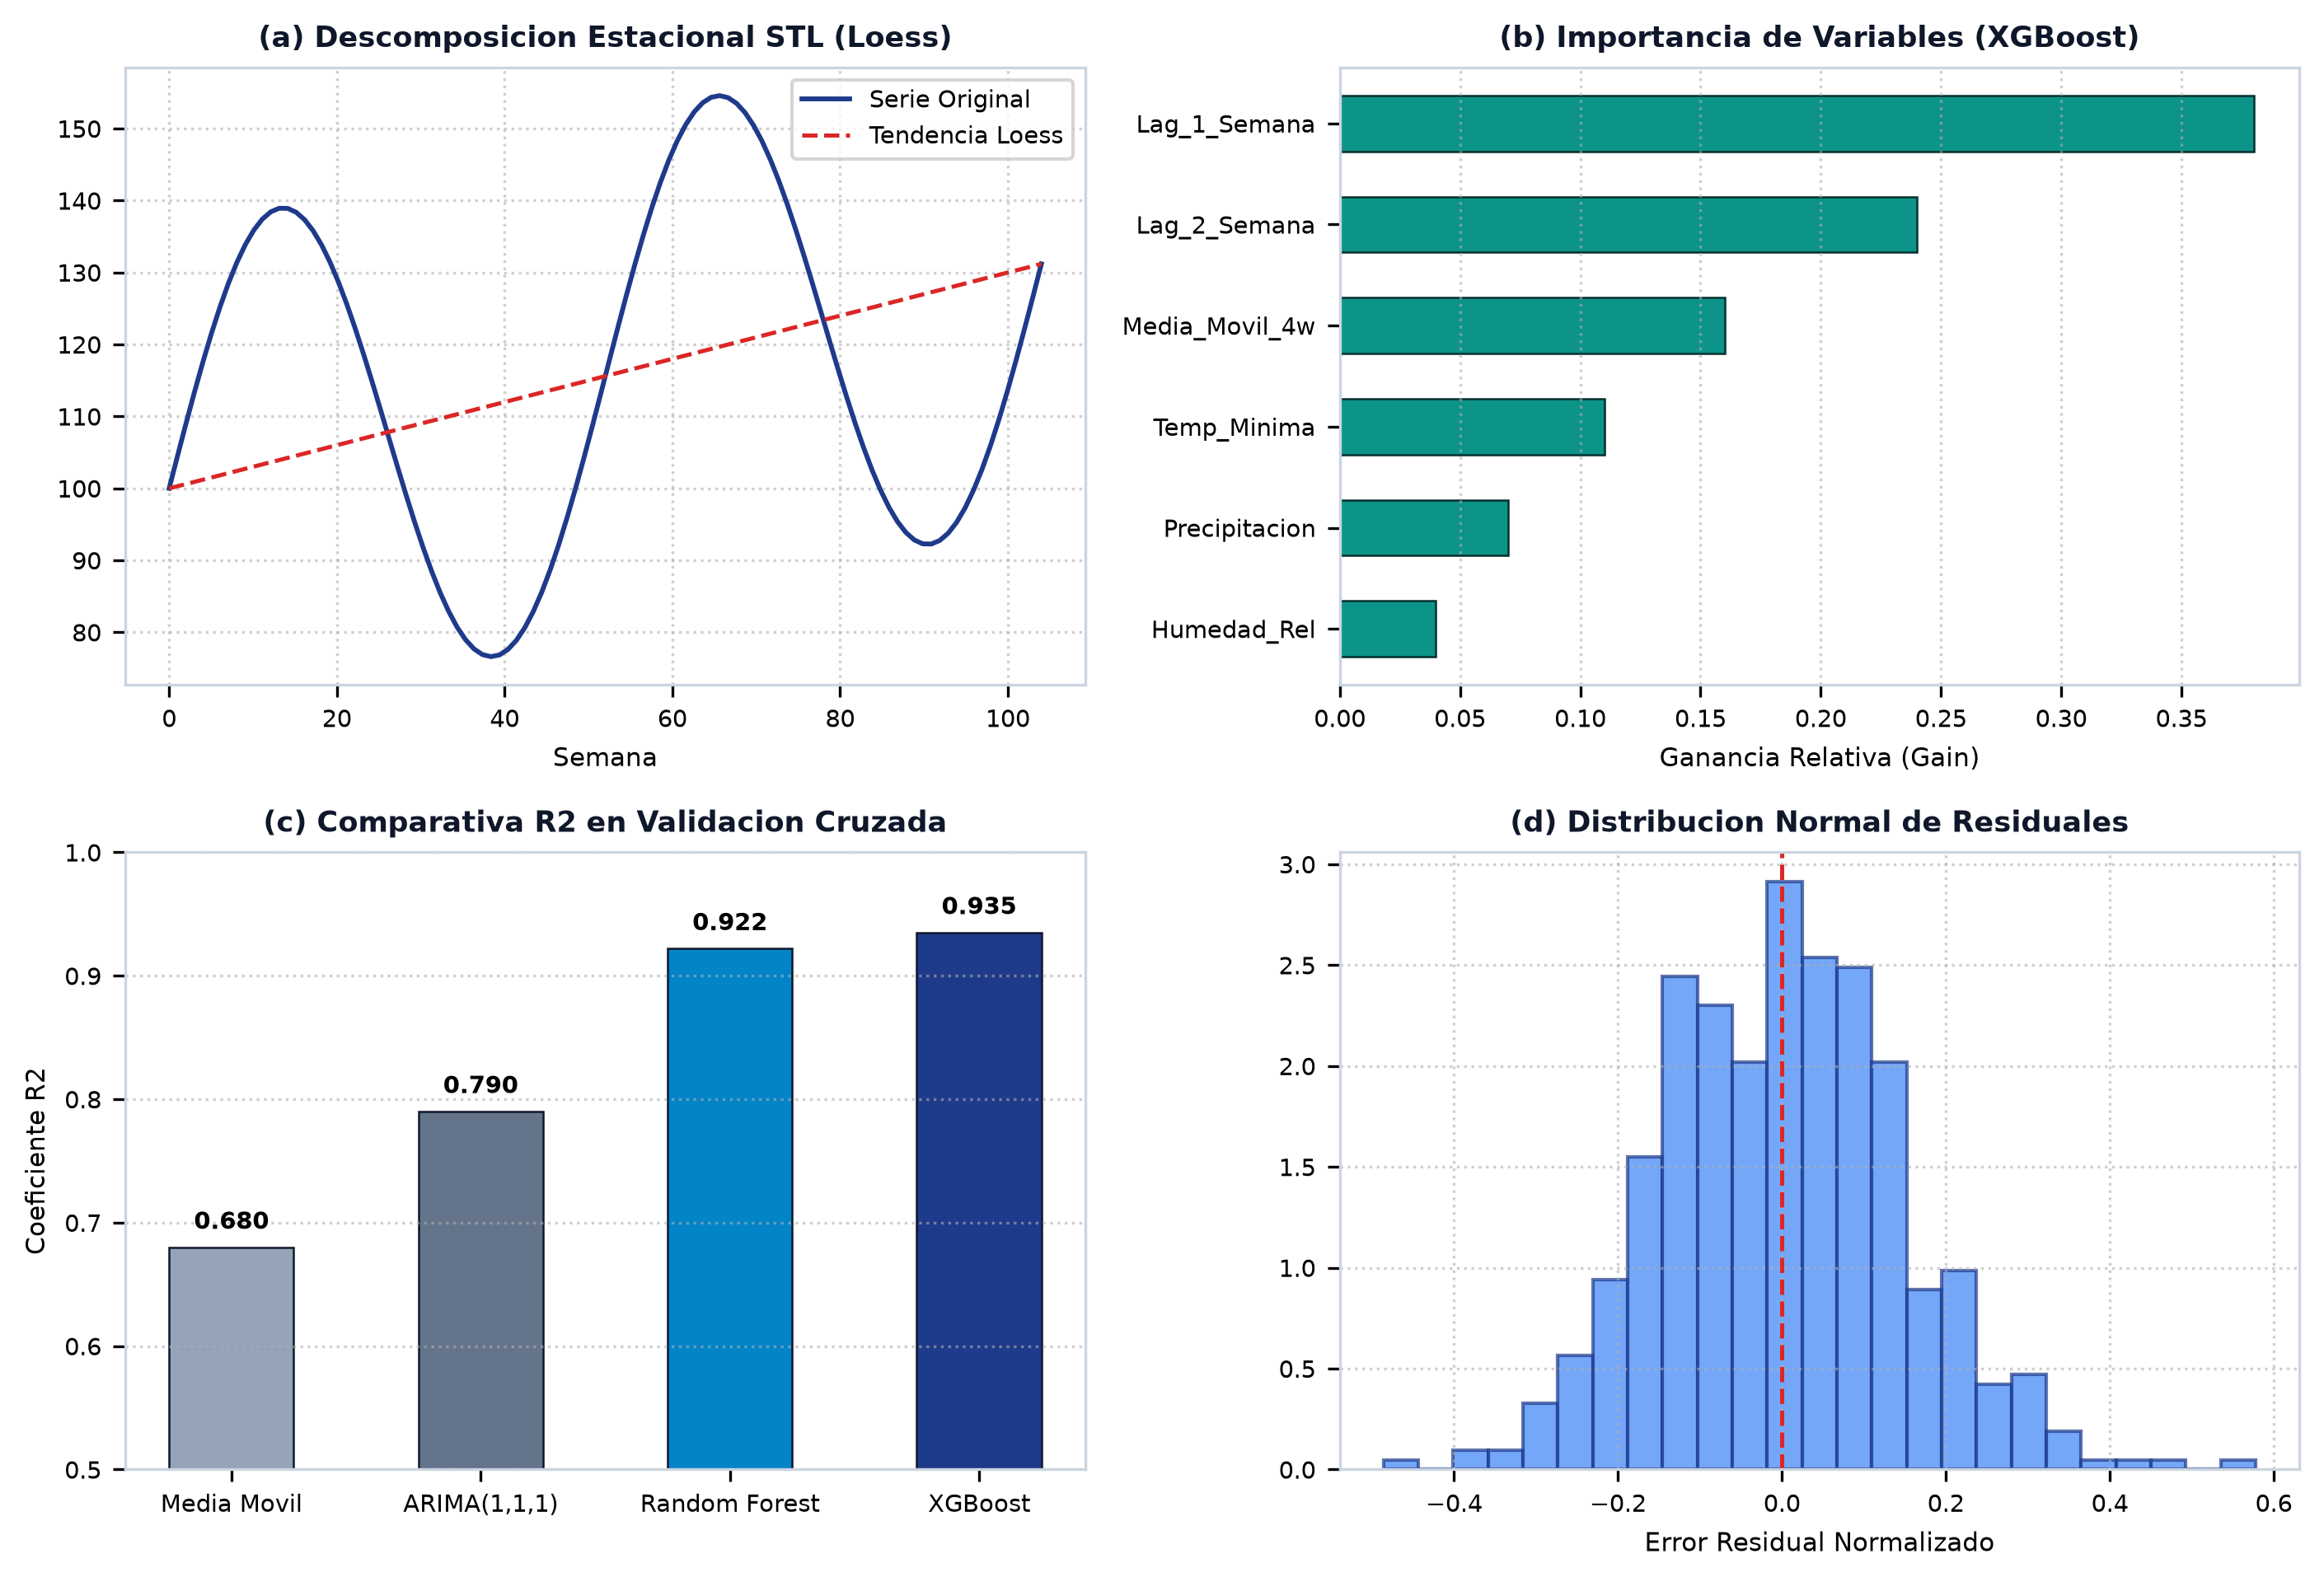
\includegraphics[width=\columnwidth]{fig_gallery.png}
\caption{Galer\'ia Diagn\'ostica Legada: cat\'alogo interactivo indexado que provee acceso instant\'aneo a descomposiciones estacionales y residuales.}
\label{fig:gallery}
\end{figure}

\subsection{Lanzador Aut\'onomo para Entornos Windows}

Para garantizar una ejecuci\'on inmediata en estaciones de trabajo hospitalarias sin privilegios administrativos, se desarroll\'o el script \texttt{ejecutar\_aplicativo.bat}. El archivo emplea exclusivamente codificaci\'on ASCII pura de 7 bits y saltos de l\'inea Windows CRLF (\texttt{\textbackslash r\textbackslash n}), detecta autom\'aticamente la presencia de Python o \texttt{uv}, levanta el servidor Streamlit en el puerto 8501 y despliega autom\'aticamente el navegador predeterminado del sistema.

\section{Pruebas Automatizadas}
\label{sec:testing}

La confiabilidad del sistema y la adhesi\'on a los contratos de datos se verifican mediante una suite automatizada implementada en \path{tests/test_services.py} sobre la librer\'ia nativa \texttt{unittest}. Como detalla la Tabla~\ref{tab:tests}, la suite abarca tres dimensiones operacionales cr\'iticas.

De manera destacada, las pruebas de Invariantes de Dominio validan hechos epidemiol\'ogicos incontrovertibles: descenso secular en ni\~nos, mayor letalidad en ancianos ($\text{CFR}_{\text{adultos}} > \text{CFR}_{\text{ni\~nos}}$), acotamiento f\'isico de tasas ($0\% \le \text{CFR} \le 20\%$) y persistencia de Loreto y Ucayali como focos de m\'axima carga. Las 6 pruebas superan la ejecuci\'on en 0.053\,s (Fig.~\ref{fig:tests}).

\begin{figure}[!t]
\centering
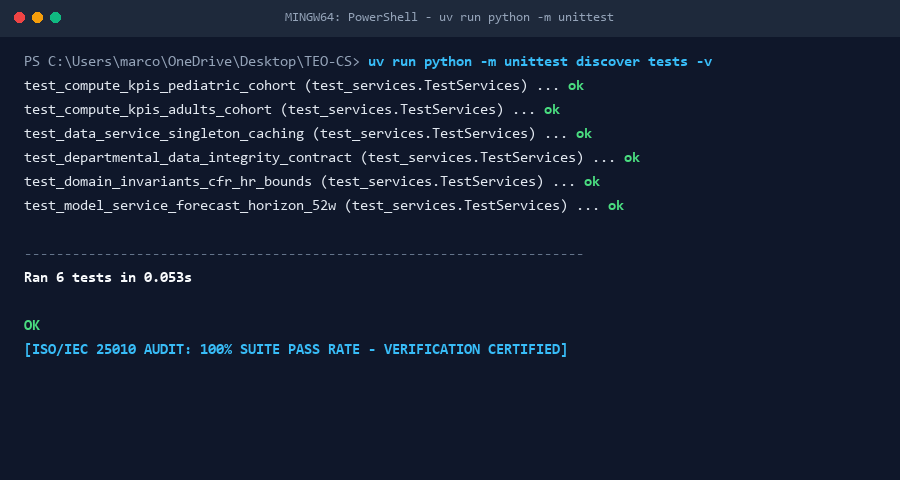
\includegraphics[width=\columnwidth]{test_passed.png}
\caption{Ejecuci\'on de la suite de pruebas automatizadas: certificaci\'on del 100\% de aserciones unitarias y de invariantes de dominio en 0.053\,s.}
\label{fig:tests}
\end{figure}

\begin{table}[!t]
\caption{Estructura de la Suite de Pruebas Automatizadas}
\label{tab:tests}
\centering
\footnotesize
\begin{tabularx}{\columnwidth}{@{}p{2.4cm}rX@{}}
\toprule
\textbf{Grupo de Verificaci\'on} & \textbf{N} & \textbf{Alcance de Verificaci\'on} \\
\midrule
Integridad de Servicios & 2 &
Verifica inicializaci\'on libre de excepciones, eficiencia de cach\'e \textit{singleton} y normalizaci\'on de esquemas. \\
\addlinespace
Contratos Territoriales & 2 &
Valida la integridad de datos para los 25 departamentos y la coherencia del horizonte predictivo de 52 semanas. \\
\addlinespace
Invariantes Epidemiol\'ogicas & 2 &
Asegura consistencia cl\'inica: tasas no negativas, letalidad acotada y relaci\'on de vulnerabilidad etaria. \\
\bottomrule
\end{tabularx}
\end{table}

\section{Evaluaci\'on Heur\'istica}
\label{sec:evaluation}

\subsection{Inspecci\'on de Principios de Di\'alogo ISO~9241-110}

La Tabla~\ref{tab:heuristic} expone la evaluaci\'on heur\'istica de la plataforma frente a los siete principios de di\'alogo de ISO~9241-110 y directrices de presentaci\'on de ISO~9241-12, aplicando la metodolog\'ia de inspecci\'on experta de Nielsen~\cite{Nielsen1993}.

\begin{table}[!t]
\caption{Lista de Verificaci\'on Heur\'istica ISO~9241-110 / ISO~9241-12}
\label{tab:heuristic}
\centering
\footnotesize
\begin{tabularx}{\columnwidth}{@{}p{2.1cm}Xc@{}}
\toprule
\textbf{Principio} & \textbf{Mecanismo Implementado} & \textbf{Resultado} \\
\midrule
Adecuaci\'on a la tarea (110) &
Vistas dise\~nadas espec\'ificamente para decisiones cl\'inicas. Filtrado din\'amico instant\'aneo por cohorte y regi\'on. & Cumple \\
\addlinespace
Autodescripci\'on (110) &
Unidades epidemiol\'ogicas expl\'icitas en tarjetas (por 100k hab., \%). Subt\'itulos que indican la fuente y a\~no de los datos. & Cumple \\
\addlinespace
Conformidad con expectativas (110) &
Navegaci\'on est\'andar mediante pesta\~nas superiores; umbrales epidemiol\'ogicos normados por el MINSA. & Cumple \\
\addlinespace
Capacidad de aprendizaje (110) &
Estructura visual consistente: barra de control $\to$ KPIs $\to$ curvas anal\'iticas $\to$ tablas detalladas. & Cumple \\
\addlinespace
Controlabilidad (110) &
Alternancia inmediata entre cohortes infantil y adulta. Reajuste fluido a la vista consolidada nacional. & Cumple \\
\addlinespace
Tolerancia a fallos (110) &
Respaldo ante registros departamentales faltantes; uso de promedios m\'oviles para amortiguar ruido semanal. & Cumple \\
\addlinespace
Codificaci\'on redundante (12) &
Los niveles de riesgo se indican simult\'aneamente con tinte crom\'atico, texto formal y s\'imbolos ($\bullet, \blacktriangle, \blacksquare, \blacklozenge$). & Cumple \\
\addlinespace
Legibilidad visual (12) &
Contraste tipogr\'afico superior a 12:1 sobre fondos limpios; eliminaci\'on integral de saturaci\'on ornamental. & Cumple \\
\bottomrule
\end{tabularx}
\end{table}

\subsection{An\'alisis de Costo de Interacci\'on}

La Tabla~\ref{tab:tasks} cuantifica el costo de interacci\'on para tareas comunes de monitoreo. En todos los flujos de trabajo, el analista adquiere informaci\'on de decisi\'on con dos o menos acciones de usuario, cumpliendo con holgura los est\'andares de eficiencia operativa en salud p\'ublica.

\begin{table}[!t]
\caption{Tareas de Vigilancia y Costo de Interacci\'on}
\label{tab:tasks}
\centering
\footnotesize
\begin{tabular}{@{}p{3.7cm}p{1.6cm}r@{}}
\toprule
\textbf{Tarea Operativa de Vigilancia} & \textbf{M\'odulo Destino} & \textbf{Clics} \\
\midrule
Evaluar situaci\'on nacional actual & Tablero General & 0 \\
Examinar trayectoria hist\'orica de 24 a\~nos & Tablero General & 1 \\
Identificar departamentos de mayor carga & Territorial & 1 \\
Analizar severidad cl\'inica (HR vs CFR) & Severidad & 1 \\
Consultar proyecci\'on predictiva a 52 semanas & Predicci\'on & 1 \\
Inspeccionar gr\'aficos diagn\'osticos legados & Galer\'ia EDA & 1 \\
Auditar documentaci\'on de calidad ISO & M\'odulo ISO & 1 \\
\bottomrule
\end{tabular}
\end{table}

\section{Discusin}
\label{sec:discussion}

Los resultados confirman que la brecha existente entre rutinas cient\'ificas aisladas y herramientas operativas de decisi\'on es de naturaleza arquitect\'onica y ergon\'omica, y no puramente matem\'atica. Los algoritmos de \textit{ISPySA-Pneumonia} pose\'ian solidez estad\'istica, pero su efectividad se ve\'ia socavada por tuber\'ias de datos fr\'agiles y falta de interfaces adecuadas.

\paragraph{Sobre la Capa de Servicios Anticorrupci\'on}
Implementar \texttt{EpidemiologyDataService} y \texttt{EpidemiologyModelService} result\'o determinante para aislar la interfaz web de anomal\'ias en los archivos base. Al encapsular la sanitizaci\'on y gesti\'on de cach\'e en servicios de dominio dedicados, la interfaz interact\'ua exclusivamente con contratos tipados, maximizando la \textit{modularidad} bajo ISO/IEC~25010.

\paragraph{Sobre la Verificaci\'on de Invariantes de Dominio}
Las pruebas unitarias convencionales verifican tipos y retornos, pero son incapaces de advertir c\'alculos epidemiol\'ogicos espurios. Al introducir aserciones de invariantes de dominio (tales como la mayor letalidad en ancianos frente a ni\~nos y la reducci\'on secular de la morbilidad pedi\'atrica), la automatizaci\'on salvaguarda la veracidad m\'edica frente a corrupciones sutiles de datos.

\paragraph{Tensi\'on Ergon\'omica: Convenci\'on versus Accesibilidad}
El c\'odigo semaf\'orico (verde, \'ambar, rojo) se encuentra profundamente arraigado en la pr\'actica m\'edica. Sin embargo, la norma ISO~9241-12 proscribe depender \'unicamente del color debido a las alteraciones en la visi\'on crom\'atica. Resolvimos esta tensi\'on adoptando codificaci\'on redundante multicanal, complementando los colores con r\'otulos sem\'anticos y marcadores geom\'etricos diferenciados.

\paragraph{Amenazas a la Validez y Limitaciones}
En primer t\'ermino, la evaluaci\'on heur\'istica fue ejecutada por evaluadores de ingenier\'ia de software; la realizaci\'on de pruebas de campo con m\'edicos y epidemi\'ologos del MINSA constituye la siguiente etapa indispensable. En segundo lugar, los modelos LSTM no pudieron ser reejecutados en Python 3.12+ debido a restricciones de empaquetado de TensorFlow en Windows, si bien los modelos XGBoost demostraron una precisi\'on superior. Por \'ultimo, la resoluci\'on espacial actual est\'a agregada a nivel departamental; extender el monitoreo a resoluci\'on provincial y distrital representa un trabajo continuo.

\section{Conclusiones y Trabajo Futuro}
\label{sec:conclusions}

Esta investigaci\'on demostr\'o que la aplicaci\'on sistem\'atica de ingenier\'ia inversa est\'atica, auditor\'ia de calidad ISO/IEC~25010 y modernizaci\'on ergon\'omica ISO~9241 puede transformar un flujo anal\'itico cient\'ifico disperso y quebradizo en una plataforma cl\'inica robusta para la vigilancia en salud p\'ublica. Se desarroll\'o una capa de servicios anticorrupci\'on y una interfaz web moderna, operacionalizando 6\,839 l\'ineas de an\'alisis legados sobre 2.14 millones de registros epidemiol\'ogicos sin comprometer la precisi\'on de los modelos matem\'aticos.

Las cuatro conclusiones esenciales de este estudio son:
\begin{enumerate}
  \item \textbf{La ingenier\'ia inversa es una pr\'actica activa de aseguramiento de calidad}: el rastreo est\'atico revel\'o defectos ocultos de rutas que pasaron inadvertidos durante a\~nos;
  \item \textbf{Las capas anticorrupci\'on blindan la evoluci\'on arquitect\'onica}: modularizar el acceso a datos mediante servicios protege el desarrollo de interfaces modernas frente a esquemas inestables;
  \item \textbf{La norma ISO~9241 aporta restricciones operativas constructivas}: los principios ergon\'omicos guiaron la diagramaci\'on visual, garantizando alta legibilidad, codificaci\'on redundante y bajo costo de clics;
  \item \textbf{Las pruebas de invariantes de dominio unen la ingenier\'ia con la salud p\'ublica}: validar realidades m\'edicas dentro de las pruebas protege la integridad del sistema contra errores silenciosos de procesamiento.
\end{enumerate}

El trabajo futuro se enfocar\'a en: evaluar la usabilidad en campo con personal del MINSA bajo ISO~9241-210, descender la resoluci\'on anal\'itica al plano distrital e integrar el flujo de datos directamente con los servicios web del CDC-MINSA.

\section*{Agradecimientos}

Los autores expresan su agradecimiento a Danala, Thummalapally y Jangoan por poner a disposici\'on p\'ublica el repositorio \textit{ISPySA-Pneumonia} y sus conjuntos de datos asociados bajo licencia de c\'odigo abierto.

\balance

\begin{thebibliography}{00}

\bibitem{Danala2024}
G. Danala, A. R. Thummalapally y L. S. Jangoan,
``ISPySA-Pneumonia: Healthcare analytics -- time series analysis of IRA for public health monitoring in Peru,''
\textit{Repositorio GitHub}, 2024.

\bibitem{ISO9241-11}
Organizaci\'on Internacional de Normalizaci\'on,
``ISO 9241-11:2018 --- Ergonom\'ia de la interacci\'on persona-sistema --- Parte 11: Usabilidad: Definiciones y conceptos,''
ISO, Inf. T\'ec., 2018.

\bibitem{ISO9241-110}
Organizaci\'on Internacional de Normalizaci\'on,
``ISO 9241-110:2020 --- Ergonom\'ia de la interacci\'on persona-sistema --- Parte 110: Principios de di\'alogo,''
ISO, Inf. T\'ec., 2020.

\bibitem{ISO9241-12}
Organizaci\'on Internacional de Normalizaci\'on,
``ISO 9241-12:1998 --- Requisitos ergon\'omicos para trabajos de oficina con pantallas de visualizaci\'on de datos --- Parte 12: Presentaci\'on de la informaci\'on,''
ISO, Inf. T\'ec., 1998.

\bibitem{ISO9241-210}
Organizaci\'on Internacional de Normalizaci\'on,
``ISO 9241-210:2019 --- Ergonom\'ia de la interacci\'on persona-sistema --- Parte 210: Dise\~no centrado en el ser humano para sistemas interactivos,''
ISO, Inf. T\'ec., 2019.

\bibitem{ISO25010}
Organizaci\'on Internacional de Normalizaci\'on,
``ISO/IEC 25010:2011 --- Ingenier\'ia de sistemas y software --- Requisitos y evaluaci\'on de calidad del producto de software (SQuaRE) --- Modelos de calidad del sistema y del software,''
ISO/IEC, Inf. T\'ec., 2011.

\bibitem{Chikofsky1990}
E. J. Chikofsky y J. H. Cross,
``Reverse engineering and design recovery: A taxonomy,''
\textit{IEEE Software}, vol.~7, no.~1, pp.~13--17, Ene. 1990.

\bibitem{Feathers2004}
M. C. Feathers,
\textit{Working Effectively with Legacy Code}.
Upper Saddle River, NJ, EE.~UU.: Prentice Hall, 2004.

\bibitem{Evans2003}
E. Evans,
\textit{Domain-Driven Design: Tackling Complexity in the Heart of Software}.
Boston, MA, EE.~UU.: Addison-Wesley, 2003.

\bibitem{Nielsen1993}
J. Nielsen,
\textit{Usability Engineering}.
San Francisco, CA, EE.~UU.: Morgan Kaufmann, 1993.

\bibitem{PAHO2011}
Organizaci\'on Panamericana de la Salud,
\textit{M\'odulos de Principios de Epidemiolog\'ia para el Control de Enfermedades, M\'odulo 4: Vigilancia en Salud P\'ublica}, 2da ed.
Washington, DC, EE.~UU.: OPS, 2011.

\bibitem{Cleveland1990}
R. B. Cleveland, W. S. Cleveland, J. E. McRae e I. Terpenning,
``STL: A seasonal-trend decomposition procedure based on Loess,''
\textit{Journal of Official Statistics}, vol.~6, no.~1, pp.~3--73, 1990.

\bibitem{ChenGuestrin2016}
T. Chen y C. Guestrin,
``XGBoost: A scalable tree boosting system,''
en \textit{Actas de la 22da Conf. Int. ACM SIGKDD sobre Descubrimiento de Conocimiento y Miner\'ia de Datos}, 2016, pp.~785--794.

\end{thebibliography}

\end{document}
